\documentclass[11pt,a4paper]{article}
\usepackage[utf8]{inputenc}
\usepackage[T1]{fontenc}
\usepackage{helvet}
\renewcommand{\familydefault}{\sfdefault}
\usepackage[margin=2.2cm]{geometry}
\usepackage{booktabs}
\usepackage{graphicx}
\usepackage{caption}
\usepackage{placeins}
\usepackage{makecell}
\usepackage{amsmath}
\usepackage{amssymb}
\usepackage{xurl}
\usepackage[super,sort&compress,comma]{natbib}
\providecommand{\nolinkurl}[1]{\url{#1}}
\providecommand{\urlprefix}{URL }
\providecommand{\doi}[1]{https://doi.org/#1}
\providecommand{\bibcommenthead}{}
\renewcommand{\bibsection}{\section*{\refname}\addcontentsline{toc}{section}{\refname}}
\captionsetup{labelfont=bf,labelsep=space,justification=raggedright,singlelinecheck=false,font=small}
\renewcommand{\tablename}{Supplementary Table}
\renewcommand{\figurename}{Supplementary Figure}
\setlength{\parindent}{0pt}\setlength{\parskip}{5.5pt}\emergencystretch=2em
\renewcommand{\topfraction}{0.9}\renewcommand{\bottomfraction}{0.8}\renewcommand{\textfraction}{0.08}\renewcommand{\floatpagefraction}{0.75}\setcounter{topnumber}{4}\setcounter{bottomnumber}{3}\setcounter{totalnumber}{6}
\makeatletter\setlength{\@fptop}{0pt}\setlength{\@fpsep}{12pt}\setlength{\@fpbot}{0pt plus 1fil}\makeatother
\begin{document}
{\large\bfseries Supplementary Information}

{\bfseries Adult gut microbiomes single out individuals at population scale}

Guillaume Gautreau\textsuperscript{1}, Guillaume Kon Kam King\textsuperscript{1}, Nicolas Pons\textsuperscript{2}, Roland Faure\textsuperscript{3}

{\small\textsuperscript{1}Université Paris-Saclay, INRAE, MaIAGE, Jouy-en-Josas, France.\\
\textsuperscript{2}Université Paris-Saclay, INRAE, MetaGenoPolis, Jouy-en-Josas, France.\\
\textsuperscript{3}CNRS UMR3525, Institut Pasteur, Université Paris Cité, Paris, 75015, France.}

{\small\setcounter{tocdepth}{3}
\renewcommand{\contentsname}{Contents}\tableofcontents
\renewcommand{\listfigurename}{Supplementary Figures}\listoffigures
\renewcommand{\listtablename}{Supplementary Tables}\listoftables}
\clearpage

\FloatBarrier
\section*{Supplementary Note 1. The cohorts}\addcontentsline{toc}{section}{Supplementary Note 1. The cohorts}

The analysis requires donors with at least two stool samples, one to query the index and another to recover among the returned runs. We searched for such donors in curatedMetagenomicData, which compiles published metagenomic studies with curated metadata. This Note describes how we selected the donors for the analysis from this resource.

\subsection*{Selection of the cohorts and donors}\addcontentsline{toc}{subsection}{Selection of the cohorts and donors}

We applied the rules below to the whole of curatedMetagenomicData, which holds 93 studies and 22,588 samples, 21,030 of them stool samples (Supplementary Fig. 1A and Supplementary Tables 1 and 2). They lead to 11 cohorts, and we left four of them out. A donor is a subject identifier of the curated metadata. We selected donors with at least two stool samples and considered their first and last samples, ordered by days since the first collection (with missing collection days assigned to day 0). A study with at least five such donors was considered a longitudinal cohort, yielding 30 cohorts comprising 2,038 donors. From here on, a donor of a cohort is a donor with at least two stool samples (but it can be more, Supplementary Fig. 1B).

\setcounter{figure}{0}
\begin{figure}[!htbp]\centering
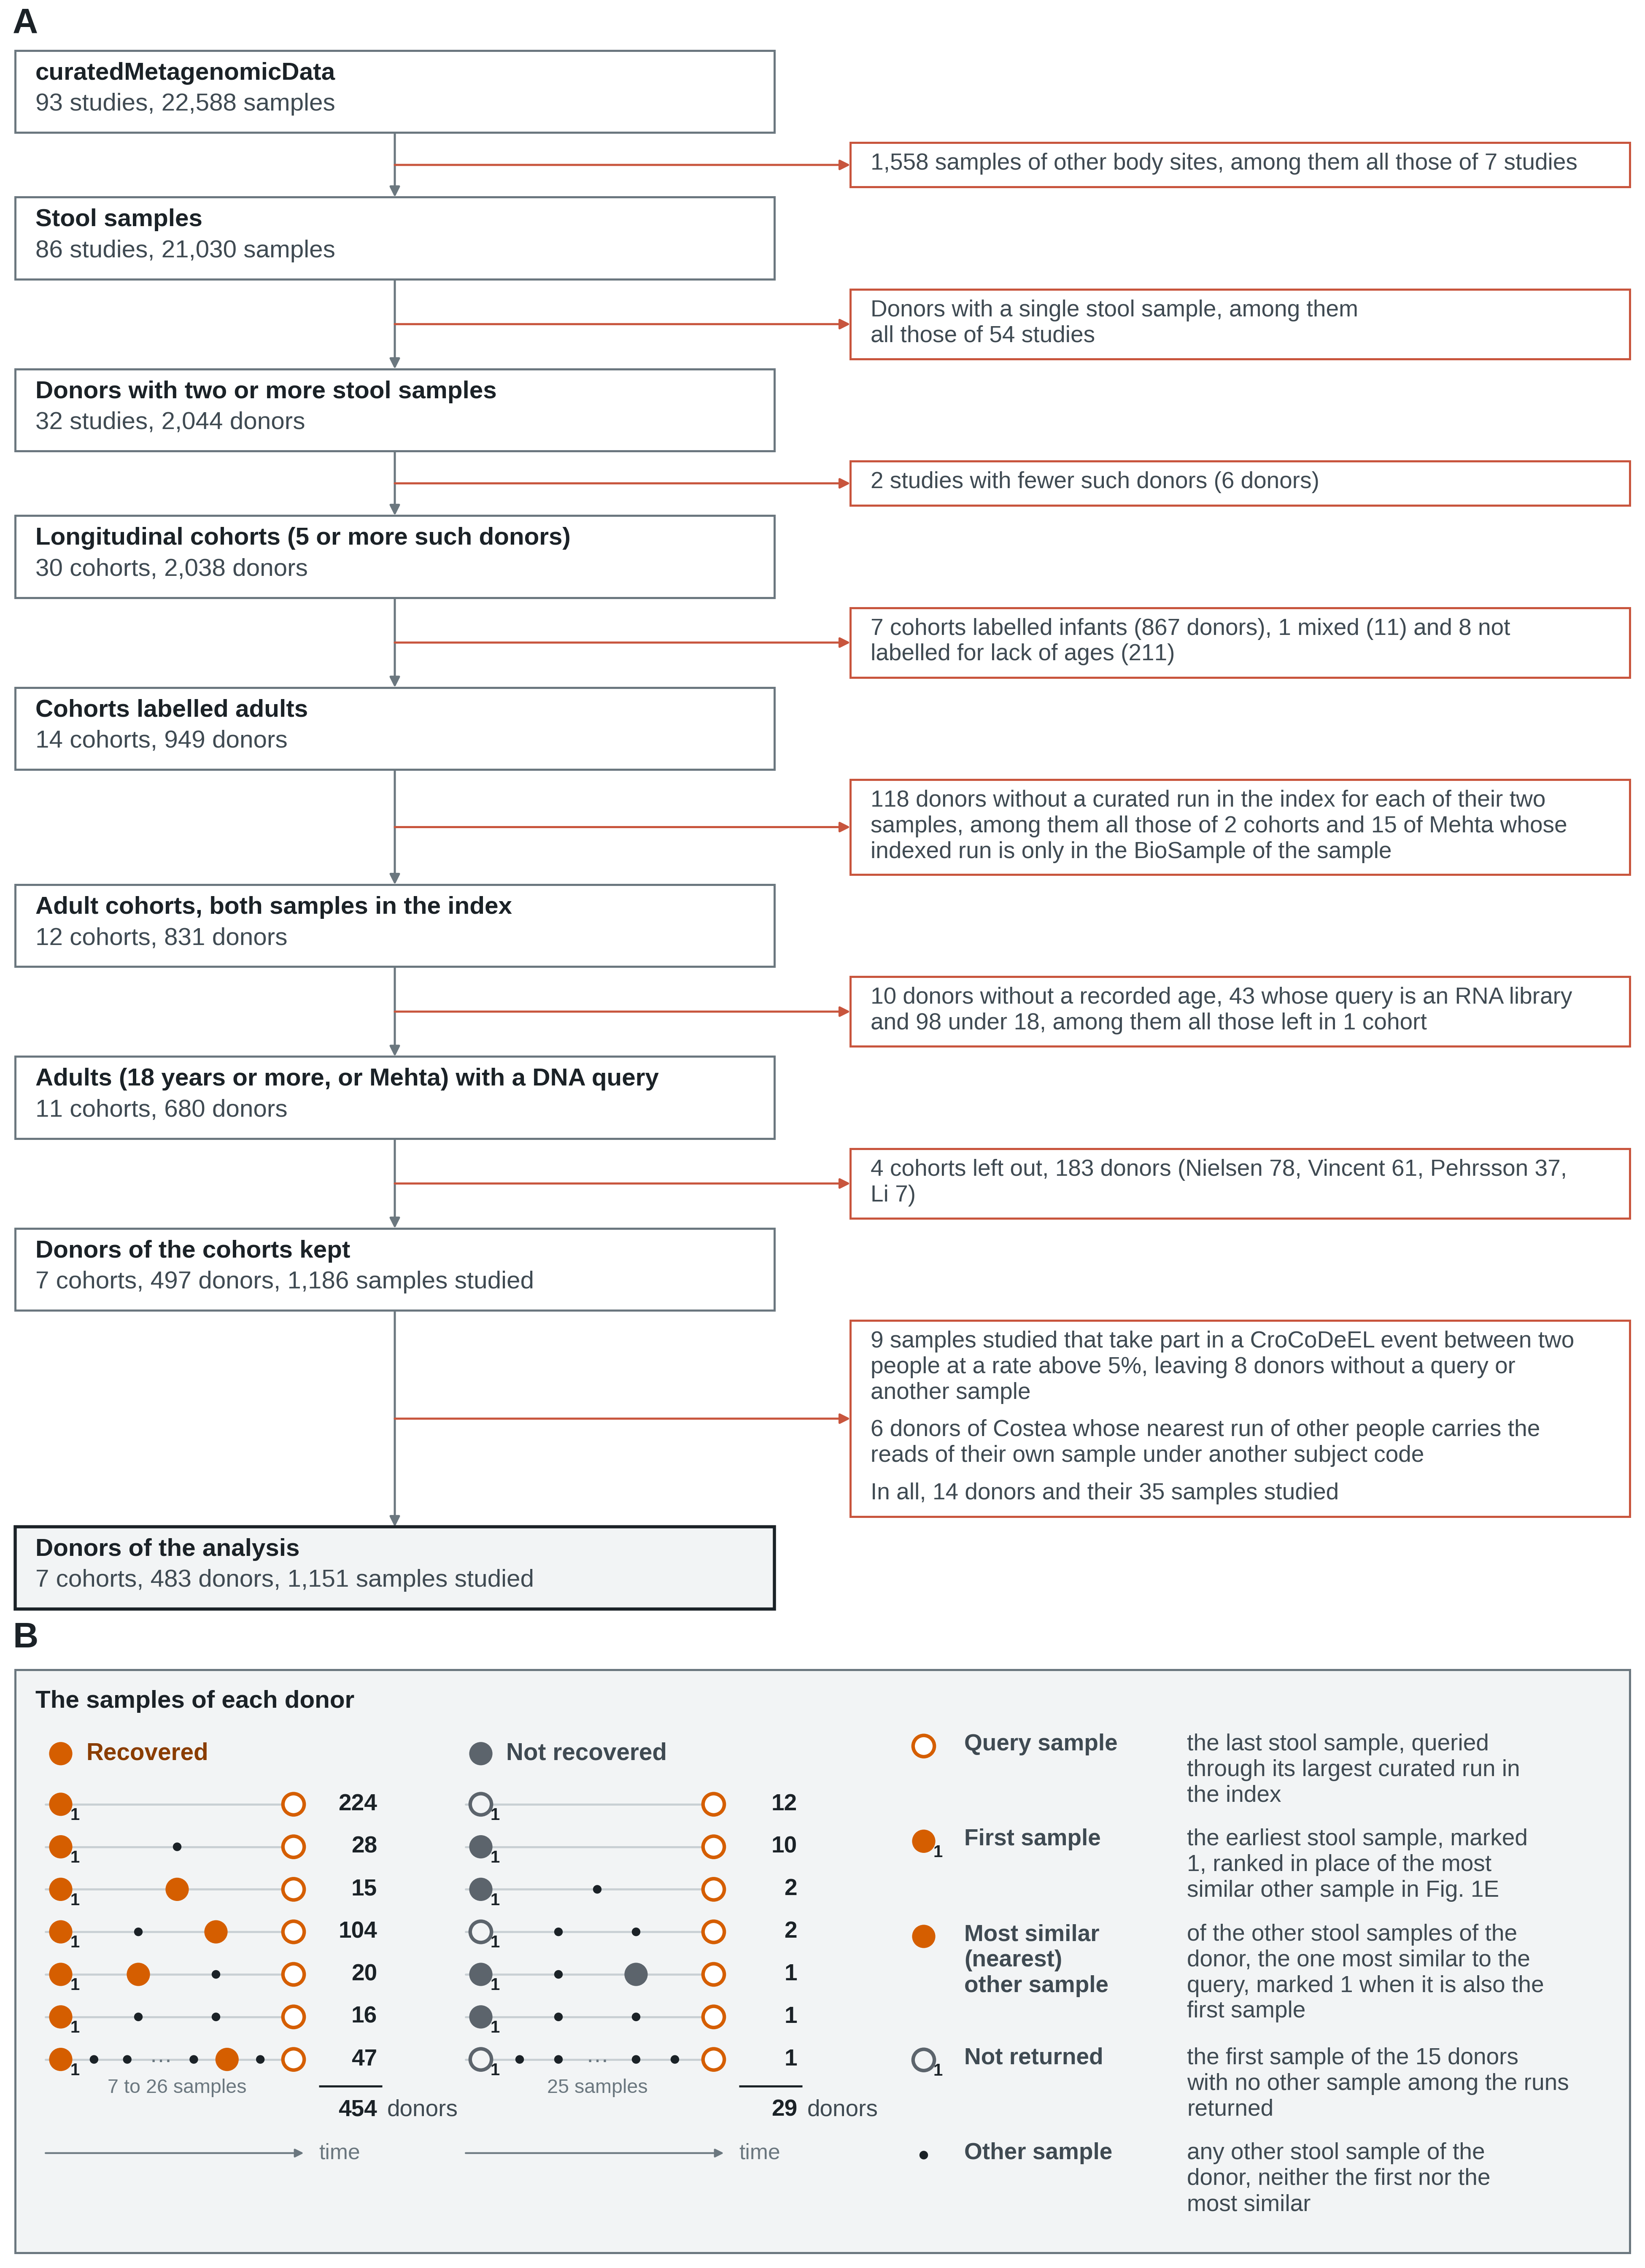
\includegraphics[width=\textwidth,height=0.79\textheight,keepaspectratio]{supplementary_figure1}
\caption[Selection of the cohorts, the donors and their samples]{\textbf{Selection of the cohorts, the donors and their samples.} \textbf{A}, From curatedMetagenomicData to the donors of the analysis, each step with the cohorts or studies and the samples or donors that it keeps (left, as in Supplementary Table 1) and what it removes (right, red; Supplementary Note 1 and Supplementary Table 2). \textbf{B}, The samples of each donor as circles along time, large for the samples studied, namely its query sample, its first sample and its most similar other sample (Supplementary Note 1), and small for its other samples. A line is one arrangement of these samples with its number of donors, left for the donors recovered and right for the others. The last line of each side stands for the donors of HMP IBD, who have 7 to 26 stool samples. A donor is a subject identifier of the curated metadata. A curated run of a sample is a run that the curated metadata list for it; HMP IBD, whose curated metadata list none, takes the runs of its project in the European Nucleotide Archive (ENA), and its first and last samples are the earliest and the latest with a run in the index.}
\end{figure}

\setcounter{table}{0}
\begin{table}[!htbp]\centering\small
\caption[Selection of the cohorts and donors of the analysis from curatedMetagenomicData]{\textbf{Selection of the cohorts and donors of the analysis from curatedMetagenomicData.} Studies and samples are those of the metadata tables of curatedMetagenomicData as of 1 October 2026. A longitudinal cohort is a study with at least 5 donors who have two or more stool samples. The pair of a donor is its first and its last stool sample, and only the last one is queried. The labels (infants, mixed, adults, not labelled) belong to the cohorts and not to their donors.}
\begin{tabular}{lrr}
\toprule
Step & Studies or cohorts & Samples or donors \\
\midrule
curatedMetagenomicData & 93 studies & 22,588 samples \\
\quad stool samples & 86 studies & 21,030 samples \\
\quad donors with two or more stool samples & 32 studies & 2,044 donors \\
\midrule
Longitudinal cohorts (5 or more such donors) & 30 cohorts & 2,038 donors \\
\quad labelled infants & 7 & 867 \\
\quad labelled mixed & 1 & 11 \\
\quad not labelled (fewer than 70\% of donors with an age) & 8 & 211 \\
\quad labelled adults & 14 & 949 \\
\midrule
Adult cohorts, both samples in the index (before Dec. 2023) & 12 cohorts & 831 donors \\
Adults (18 years or more, or Mehta) with a DNA query & 11 cohorts & 680 donors \\
Without the 4 cohorts left out & 7 cohorts & 497 donors \\
Without the 14 donors removed by two rules & 7 cohorts & 483 donors \\
\bottomrule
\end{tabular}
\end{table}

\setcounter{table}{1}
\begin{table}[!htbp]\centering\footnotesize\setlength{\tabcolsep}{3pt}
\caption[Selection of the donors of the analysis in each of the 14 adult cohorts]{\textbf{Selection of the donors of the analysis in each of the 14 adult cohorts.} \textit{Donors}, donors with two or more stool samples in the curated metadata. \textit{In the index}, each of the two samples of the donor has a run in the 4,791,208 runs of the index (Logan v1.1 freeze of the Sequence Read Archive, last updated in December 2023, with a new update in progress), among the runs that the curated metadata list for the sample (for HMP IBD, among the runs of its ENA project; Supplementary Note 1). \textit{Under 18}, the lowest recorded age of the donor is under 18. \textit{No age}, no age is recorded; Mehta records none, but its donors are not counted here (Supplementary Note 1). \textit{RNA}, the queried run is named as an RNA library. \textit{Adults, DNA} (donors in the index that are in none of these three columns). \textit{Removed}, donors of the cohorts kept removed by the rule of contamination and by that of re-deposit, in this order (Supplementary Note 1). \textit{In the analysis}, the donors of the 7 cohorts kept that the two rules leave. \textit{Women/men}, the women and the men among the donors of the analysis, by the sex that the curated metadata record. \textit{Country}, the country that the curated metadata record for these donors.}
\begin{tabular}{lrrrrrrrrrl}
\toprule
Cohort & Donors & \makecell[rb]{In the\\index} & \makecell[rb]{Under\\18} & \makecell[rb]{No\\age} & RNA & \makecell[rb]{Adults,\\DNA} & Removed & \makecell[rb]{In the\\analysis} & \makecell[rb]{Women/\\men} & Country \\
\midrule
\multicolumn{11}{l}{\textit{Cohorts kept}} \\
Mehta & 300 & 285 & -- & -- & 43 & 242 & 1 + 0 & 241 & 0/241 & United States \\
HMP IBD & 111 & 100 & 51 & 1 & -- & 48 & -- & 48 & 26/22 & United States \\
Costea & 107 & 107 & 7 & 9 & -- & 91 & 1 + 6 & 84 & 54/30 & Kazakhstan \\
Hansen & 52 & 46 & -- & -- & -- & 46 & 2 + 0 & 44 & 24/20 & Denmark \\
Bengtsson-Palme & 35 & 33 & -- & -- & -- & 33 & 4 + 0 & 29 & 23/6 & Sweden \\
Raymond & 24 & 24 & -- & -- & -- & 24 & -- & 24 & 13/11 & Canada \\
Heintz-Buschart & 20 & 20 & 7 & -- & -- & 13 & -- & 13 & 9/4 & Luxembourg \\
\midrule
\multicolumn{11}{l}{\textit{Cohorts left out (Supplementary Note 1)}} \\
Nielsen & 78 & 78 & -- & -- & -- & 78 & -- & 0 & -- & \multicolumn{1}{c}{--} \\
Vincent & 69 & 61 & -- & -- & -- & 61 & -- & 0 & -- & \multicolumn{1}{c}{--} \\
Pehrsson & 59 & 59 & 22 & -- & -- & 37 & -- & 0 & -- & \multicolumn{1}{c}{--} \\
Li & 7 & 7 & -- & -- & -- & 7 & -- & 0 & -- & \multicolumn{1}{c}{--} \\
\midrule
\multicolumn{11}{l}{\textit{Cohorts without a donor to analyse}} \\
HMP 2012 & 47 & 0 & -- & -- & -- & 0 & -- & 0 & -- & \multicolumn{1}{c}{--} \\
HMP 2019 T2D & 28 & 0 & -- & -- & -- & 0 & -- & 0 & -- & \multicolumn{1}{c}{--} \\
Ijaz & 12 & 11 & 11 & -- & -- & 0 & -- & 0 & -- & \multicolumn{1}{c}{--} \\
\midrule
All 14 adult cohorts & 949 & 831 & 98 & 10 & 43 & 680 & 8 + 6 & 483 & 149/334 & 6 countries \\
\bottomrule
\end{tabular}
\end{table}

We then labelled each cohort by the ages that the curated metadata record for its donors at their first sample. A donor under 3 years is an infant. A cohort is labelled when at least 70\% of its donors have an age. It is labelled as infants if at least 80\% of the donors with an age are infants, as adults if at most 20\% of them are, and as mixed otherwise. The label belongs to the cohort and not to its donors, so an adult cohort can hold minors, which the age rule below removes. Mehta records no age, but all its stool samples are from men and the study describes a cohort of adult men\cite{mehta2018}, so we counted it as adult. This gives 7 infant cohorts (867 donors), 14 adult cohorts (949), 1 mixed cohort (11) and 8 cohorts that could not be labelled for lack of ages (211). We kept the adult cohorts, because the question is the linking of one adult, and did not query the infant cohorts. The 8 cohorts without enough ages were not queried either. The curated age category marks all the stool samples of 5 of them (84 donors) as adult. However, this category is filled even when no age is recorded, and these 5 cohorts record no age, so we did not count them as adult.

A donor of the 14 adult cohorts is analysed only if each of its two samples has a run in the index. This run must be among the runs listed in the curated metadata or, for HMP IBD, whose curated metadata list none, among the runs of its ENA project (below). This index rule holds for 831 donors in 12 cohorts, 100 of them in HMP IBD. Another 15 donors of Mehta have an indexed run of each sample, but for at least one of the two samples this run is in the BioSample of the sample without being among its curated accessions. These donors are left out. 20 donors that this rule leaves out were queried all the same, because the curated run of their last sample is indexed. Their lists of neighbours only complete the HGM set (Supplementary Table 3), and no rank of the analysis depends on them. Supplementary Table 4 gives the results with other sets of runs counted as other people. Two cohorts could not be tested. None of the reads of HMP 2012 (47 donors) is in the index, and the ENA lists them as controlled access (dbGaP). The curated samples of HMP 2019 T2D (28 donors) carry no run accession and its ENA project holds only amplicon runs. HMP IBD has no run accession in the curated metadata either, so we took the first and the last sample of each of its donors from its ENA project. This was possible for 103 of its 111 donors, those with at least two collection dates among the metagenomic runs of the project whose sample alias is a participant and visit code without suffix. For 100 of these 103, the first and the last of these dates each have one of these runs in the index. In the ENA project a sample is a visit of a participant. A visit counts as a curated sample when a curated sample of the donor has twice the read count of one of the ENA runs of the visit, because the curated metadata count both reads of a read pair where the ENA counts the read pair once. For the 48 of these 100 donors that stay in the analysis after the age rule below, the first and last samples are the earliest and the latest of the visits that have such a run in the index. The query is the deepest of these runs for the last visit. Fig. 1E uses these first and last samples. In the 30-day subset (Methods) the query is the same and the place of the other sample is taken by the most similar of the donor's visits at least 30 days from the query that have a run in the index.

\setcounter{table}{2}
\begin{table}[!htbp]\centering\small
\caption[Composition of the HGM set, the runs of the index taken as human gut metagenomes]{\textbf{Composition of the HGM set, the runs of the index taken as human gut metagenomes.} \textit{Labelled}, human gut or faecal shotgun metagenome in the Logan metadata. These runs include none of the indexed runs of Costea, Hansen and Raymond, which are deposited under \textit{Homo sapiens}, feces metagenome and gut metagenome respectively. \textit{Curated}, the other runs that curatedMetagenomicData lists for its stool samples or that belong to the BioSamples of the stool samples of the 7 cohorts, kept when the ENA gives them a metagenomic library of strategy WGS, WGA or OTHER. \textit{Neighbours}, the other runs that are among the 5,000 nearest runs of at least one of the 851 stool queries (those of the 831 donors in the index and of 20 more; Supplementary Note 1) and that have a metagenomic library of strategy WGS, WGA or OTHER, one of the organism labels of the rows below, no declared non-human host and no other part of the body as declared source (ENA, November 2026). \textit{Other gut or feces labels}, the other runs of the index whose organism label at the ENA is gut metagenome, feces metagenome, human gut metagenome or human feces metagenome, with the same conditions on the library, the host and the source as the neighbours. These runs are in no list of neighbours, so they change no rank, only the size of the pools.}
\begin{tabular}{lr}
\toprule
Runs & Number \\
\midrule
Labelled & 172,075 \\
Curated & 13,232 \\
Neighbours & 69,835 \\
\quad gut or feces metagenome & 20,057 \\
\quad human metagenome & 12,476 \\
\quad metagenome, human host declared & 10,427 \\
\quad metagenome, no host declared & 10,219 \\
\quad \textit{Homo sapiens} & 9,453 \\
\quad human gut or feces metagenome, library other than WGS & 7,195 \\
\quad human gut or feces metagenome, WGS & 8 \\
Other gut or feces labels & 36,739 \\
\quad gut or feces metagenome & 17,502 \\
\quad human gut or feces metagenome, library other than WGS & 19,172 \\
\quad human gut or feces metagenome, WGS & 65 \\
\midrule
All & 291,881 \\
\bottomrule
\end{tabular}
\end{table}

\setcounter{table}{3}
\begin{table}[!htbp]\centering\footnotesize\setlength{\tabcolsep}{4pt}
\caption[Sensitivity of the results to the set of runs counted as other people]{\textbf{Sensitivity of the results to the set of runs counted as other people.} Each row counts only the runs of the set as other people. \textit{Recovered}, donors for whom no run of the set has higher similarity to the query than their other sample. \textit{Threshold}, the similarity at which as many searches for an absent person are accepted as donors present are rejected (equal error rate, Fig. 1H). \textit{Error}, the share of the 483 searches for an absent person that are accepted at the threshold, equal to the share of the 483 donors present that are rejected, in \%. \textit{Accepted, recovered} (donors whose other sample reaches the threshold and who are recovered, \% of 483). \textit{Straight line}, the value at $8\times10^9$, in \%, of the straight line of Fig. 1B fitted again with the ranks among the runs of the set. The pools are drawn from $M$ = 291,881 runs, the size of the HGM set, whatever the size of the set, except in the last row ($M$ = 172,075, the labelled runs). Four projects each hold people of one of the 7 cohorts. The runs of PRJNA306874 and PRJNA389280 that the public table of the HMP consortium gives to a donor count as that donor's own (Supplementary Note 1), and the other runs of the four projects count as other people in the first row. The three rows that remove the four projects keep the runs of PRJEB41102 (Supplementary Note 1), and the rule of re-deposit of Supplementary Note 1 removes the donors whose nearest run of other people is one of these runs. PRJEB24041 deposits again the reads of part of Costea (338 of its 633 runs carry the name of a Costea sample), PRJEB28237 holds cultures of the stool of the donors of Raymond (same subject codes), PRJNA306874 (``iHMP ibdmdb'') has sample titles that carry the curated sample identifiers of HMP IBD, and PRJNA389280 is a second deposit of the metagenomes of HMP IBD, whose sample aliases the table of the consortium names.}
\begin{tabular}{lrrrrrr}
\toprule
Runs & Number & Recovered & Threshold & Error & \makecell[rb]{Accepted,\\recovered} & Straight line \\
\midrule
The HGM set (the paper) & 291,881 & 454 & 0.2338 & 12.2 & 423 (87.6) & 90.7 \\
Without PRJEB24041 and PRJEB28237 & 290,425 & 454 & 0.2331 & 12.2 & 423 (87.6) & 90.7 \\
Also without PRJNA306874 & 290,150 & 454 & 0.2331 & 12.2 & 423 (87.6) & 90.7 \\
Also without PRJNA389280 & 289,859 & 454 & 0.2318 & 12.2 & 423 (87.6) & 90.7 \\
All the runs of the index & 4,791,208 & 454 & 0.2347 & 12.4 & 422 (87.4) & 90.8 \\
Runs labelled human gut or faecal & 172,075 & 454 & 0.2318 & 12.2 & 423 (87.6) & 90.2 \\
\bottomrule
\end{tabular}
\end{table}

Two donor rules select the donors of these cohorts. The first keeps the donors with a lowest recorded age of 18 years or more and those of Mehta, which records no age and was counted as adult (above). Of the 831 donors it removes 98 under 18 and 10 without an age. The 98 donors under 18 include the 11 donors of Ijaz that are in the index (all its donors are aged 7 to 14), so this cohort leaves the analysis. The second rule requires a DNA query. It removes the 43 donors of Mehta whose queried run is named as an RNA library (a library name ending in \_rna). Of these 43 donors, 20 are recovered (47\%; rank 1 among all the runs of the index), compared with 228 of the 242 donors of Mehta with a DNA query (94\%). The rule looks at the query only. For 3 donors of Mehta that stay in the analysis, the curated metadata name only RNA libraries for the first sample and for every other sample at least 30 days from the query. The DNA library of each of these samples is recognised as a run of the donor (Methods). The two donor rules leave 680 donors in 11 cohorts. Without the four cohorts left out and the 14 donors that the rules of contamination and re-deposit remove (below), the analysis holds 483 donors in 7 cohorts (Supplementary Table 2).

\subsection*{Cohorts left out}\addcontentsline{toc}{subsection}{Cohorts left out}

Four of the 11 cohorts that the rules lead to were left out of the analysis, for the reasons below. With these four cohorts included, the analysis would hold 666 donors in 11 cohorts, and 78.2\% of them would be recovered (rank 1 among all the runs of the index).

\subsubsection*{Pehrsson}\addcontentsline{toc}{subsubsection}{Pehrsson}

Its 191 samples include pairs of samples that come from two different participants and have near-identical species profiles, so the sample of a participant is not always that participant's. The cohort was left out for these profiles.

In this cohort, 42 of the 18,007 pairs of samples from two participants have a Bray-Curtis dissimilarity below 0.10 (e.g., samples 010202 and 020202, corresponding to SAMN04261148, participant 1\_2, 68-year-old female and SAMN04261163, participant 2\_2, 4-year-old female, both 7 days after the first collection, have a dissimilarity of 0.04). The median dissimilarity is 0.71 over all these pairs and 0.50 between two samples of one participant. Of the 106 events that CroCoDeEL reports in this cohort (below), 105 are between two participants (median rate 80\%, median dissimilarity of their two samples 0.06), against 43 of the 645 events of all the samples of the 7 cohorts kept. Of the 16 adult donors of this cohort whose query sample is in one of these 42 pairs, 15 have as nearest run of the index, once the runs of the query sample itself are set aside, a run of the sample of the other participant of the pair (median similarity 0.35). This run is more similar than every other sample of the donor among the runs returned. For 14 of these 15 donors at least one such sample is returned, and the most similar one has a similarity of 0.18 at the median. None of the 16 donors is recovered.

We located these pairs in the sequencing lanes (Supplementary Table 5). Each sample has an unpaired run whose name in the SRA carries a date and, for 135 of the 191 samples, a lane. None of the 42 pairs spans two lanes. When the samples of a lane are ordered by the accession of their unpaired run, 32 of the 36 pairs that sit inside the 6 named lanes join samples exactly 12 positions apart. Of the 63 pairs of samples from two participants that are 12 positions apart in these lanes, 32 are below 0.10, compared with 0 of the 308 pairs that are 1, 2, 11 or 13 positions apart. The other 6 of the 42 pairs are inside the sequencing run dated 140805, which has no lane name. The Methods of Pehrsson \textit{et al.}\cite{pehrsson2016} report demultiplexing by barcode with no mismatches, with reads whose pair did not carry the same barcode kept as unpaired reads.

\setcounter{table}{4}
\begin{table}[!htbp]\centering\small
\caption[Pairs of samples of different participants with near-identical profiles in Pehrsson, by sequencing lane]{\textbf{Pairs of samples of different participants with near-identical profiles in Pehrsson, by sequencing lane.} \textit{Lane}, the date and the lane named in the SRA alias of the unpaired run of each sample. The position of a sample in a lane is the rank of the accession of that run among the samples of the lane. \textit{Samples}, samples of the cohort in the lane. \textit{Pairs 12 apart}, pairs of samples of different participants 12 positions apart; \textit{below 0.10}, those with a Bray-Curtis dissimilarity below 0.10. \textit{Any distance}, pairs of samples of different participants with a Bray-Curtis dissimilarity below 0.10 inside the lane, whatever the number of positions between them.}
\begin{tabular}{lrrrr}
\toprule
Lane & Samples & Pairs 12 apart & Below 0.10 & Any distance \\
\midrule
141118, lane 1 & 24 & 12 & 10 & 10 \\
141118, lane 2 & 24 & 12 & 11 & 11 \\
150102, lane 1 & 24 & 12 & 4 & 4 \\
150102, lane 2 & 19 & 7 & 4 & 5 \\
150102, lane 3 & 20 & 8 & 0 & 3 \\
150102, lane 4 & 24 & 12 & 3 & 3 \\
140805 (no lane name) & 40 & 28 & 1 & 6 \\
\midrule
All rows above (175 of 191 samples) & 175 & 91 & 33 & 42 \\
\bottomrule
\end{tabular}
\end{table}

Of the 37 adult donors of this cohort, 22 have the query sample or the other sample in one of the 42 pairs below 0.10; 1 of them is recovered, compared with 3 of the 15 others.

Although the cause cannot be clearly established from the public data, this pattern may result from a mixing of DNA or barcodes between two sets of 12 libraries of a lane during library preparation. We left this cohort out of the analysis as a precaution. The corresponding author of Pehrsson \textit{et al.} was informed of these observations on 17 November 2026 and is looking into the matter. The authors were able to reproduce the near-identical profiles and to confirm the issue (e-mail from the second author, 23 November 2026).

\subsubsection*{Nielsen and Li}\addcontentsline{toc}{subsubsection}{Nielsen and Li}

These two cohorts carry the same subject identifiers for 44 patients. The samples that the two cohorts hold under one identifier are different samples with different run accessions, two in Nielsen and a third in Li for 35 of the 44 identifiers (below). For 34 of the 78 Nielsen donors, the 5,000 nearest runs of the query include a sample of Li under the same identifier. The pipeline counts such a sample as another person, so it can have higher similarity to the query than the donor's other sample. The 35 Nielsen donors whose other sample is at rank 2 or more are only in part the 35 donors with a sample in Li. Of these 35 donors, 24 have a run of Li as the nearest run of other people, 21 of them under the donor's own identifier. We then counted a sample of the other cohort that carries the donor's identifier as a sample of the donor and not as another person. With this counting, 61 of the 78 Nielsen donors are recovered instead of 37, and 4 of the 7 Li donors instead of 3. Nielsen also shares 177 identifiers with LeChatelier 2013, a cohort of the same consortium that is not in the analysis and whose runs the pipeline cannot assign to a person. These numbers are therefore lower bounds. We left both cohorts out rather than merge identifiers across cohorts that we cannot all resolve.

These recovered links nevertheless indicate that a person's samples can be recovered across two studies that differ in instrument, read length and depth (below).

The 44 patients all have inflammatory bowel disease and come from the Spanish MetaHIT collection. For 35 of the 44 patients Nielsen holds two samples (time points 0 and 2, by their names) and Li one (time point 1). The other 9 patients have a single Nielsen sample and one Li sample, and one of them has a second Li sample. The dates of the Li samples are not recorded. The samples of the two cohorts were deposited in two studies (ENA projects PRJEB1220 for Nielsen and PRJEB5224 for Li), which share no run accession, no sample accession and no library name. The supplementary table of Li lists the Nielsen samples of these individuals under the same individual code. Of the 78 Nielsen donors, 35 are among these patients.

When a Nielsen donor queries the index, the Li sample with the same identifier is the nearest run of the HGM set for 29 of the 35 donors, apart from the donor's own Nielsen samples. It is among the 5,000 nearest runs that the Faure \textit{et al.}\cite{faure2026} service returns for 34 of the 35 (Supplementary Fig. 2A). In the other direction, when the 45 Li samples of the 44 patients query the index, 41 of them find a Nielsen sample of their identifier first. For 29 of the 35 donors the sample of the other cohort is first in both directions. When the 35 Nielsen donors query the index, the Li sample is more similar to the query than the donor's own other sample for 25 of them. The median similarity to the query is 0.40 for the Li sample, 0.30 for the donor's own other sample and 0.21 for the nearest run of other people when the Li sample of the same identifier is not counted as one (Supplementary Fig. 2B). The highest similarity between a query and a sample of the same identifier in the other cohort, in either direction, is 0.67, below the 0.78 to 0.89 found between a run and the same reads deposited again, less trimmed and filtered (below), and far from the 0.99 at which the pipeline removes a run as a quasi-exact re-deposit. With the Li sample counted as another person, the donor's other sample is first for only 8 of these 35 donors.

\setcounter{figure}{1}
\begin{figure}[!htbp]\centering
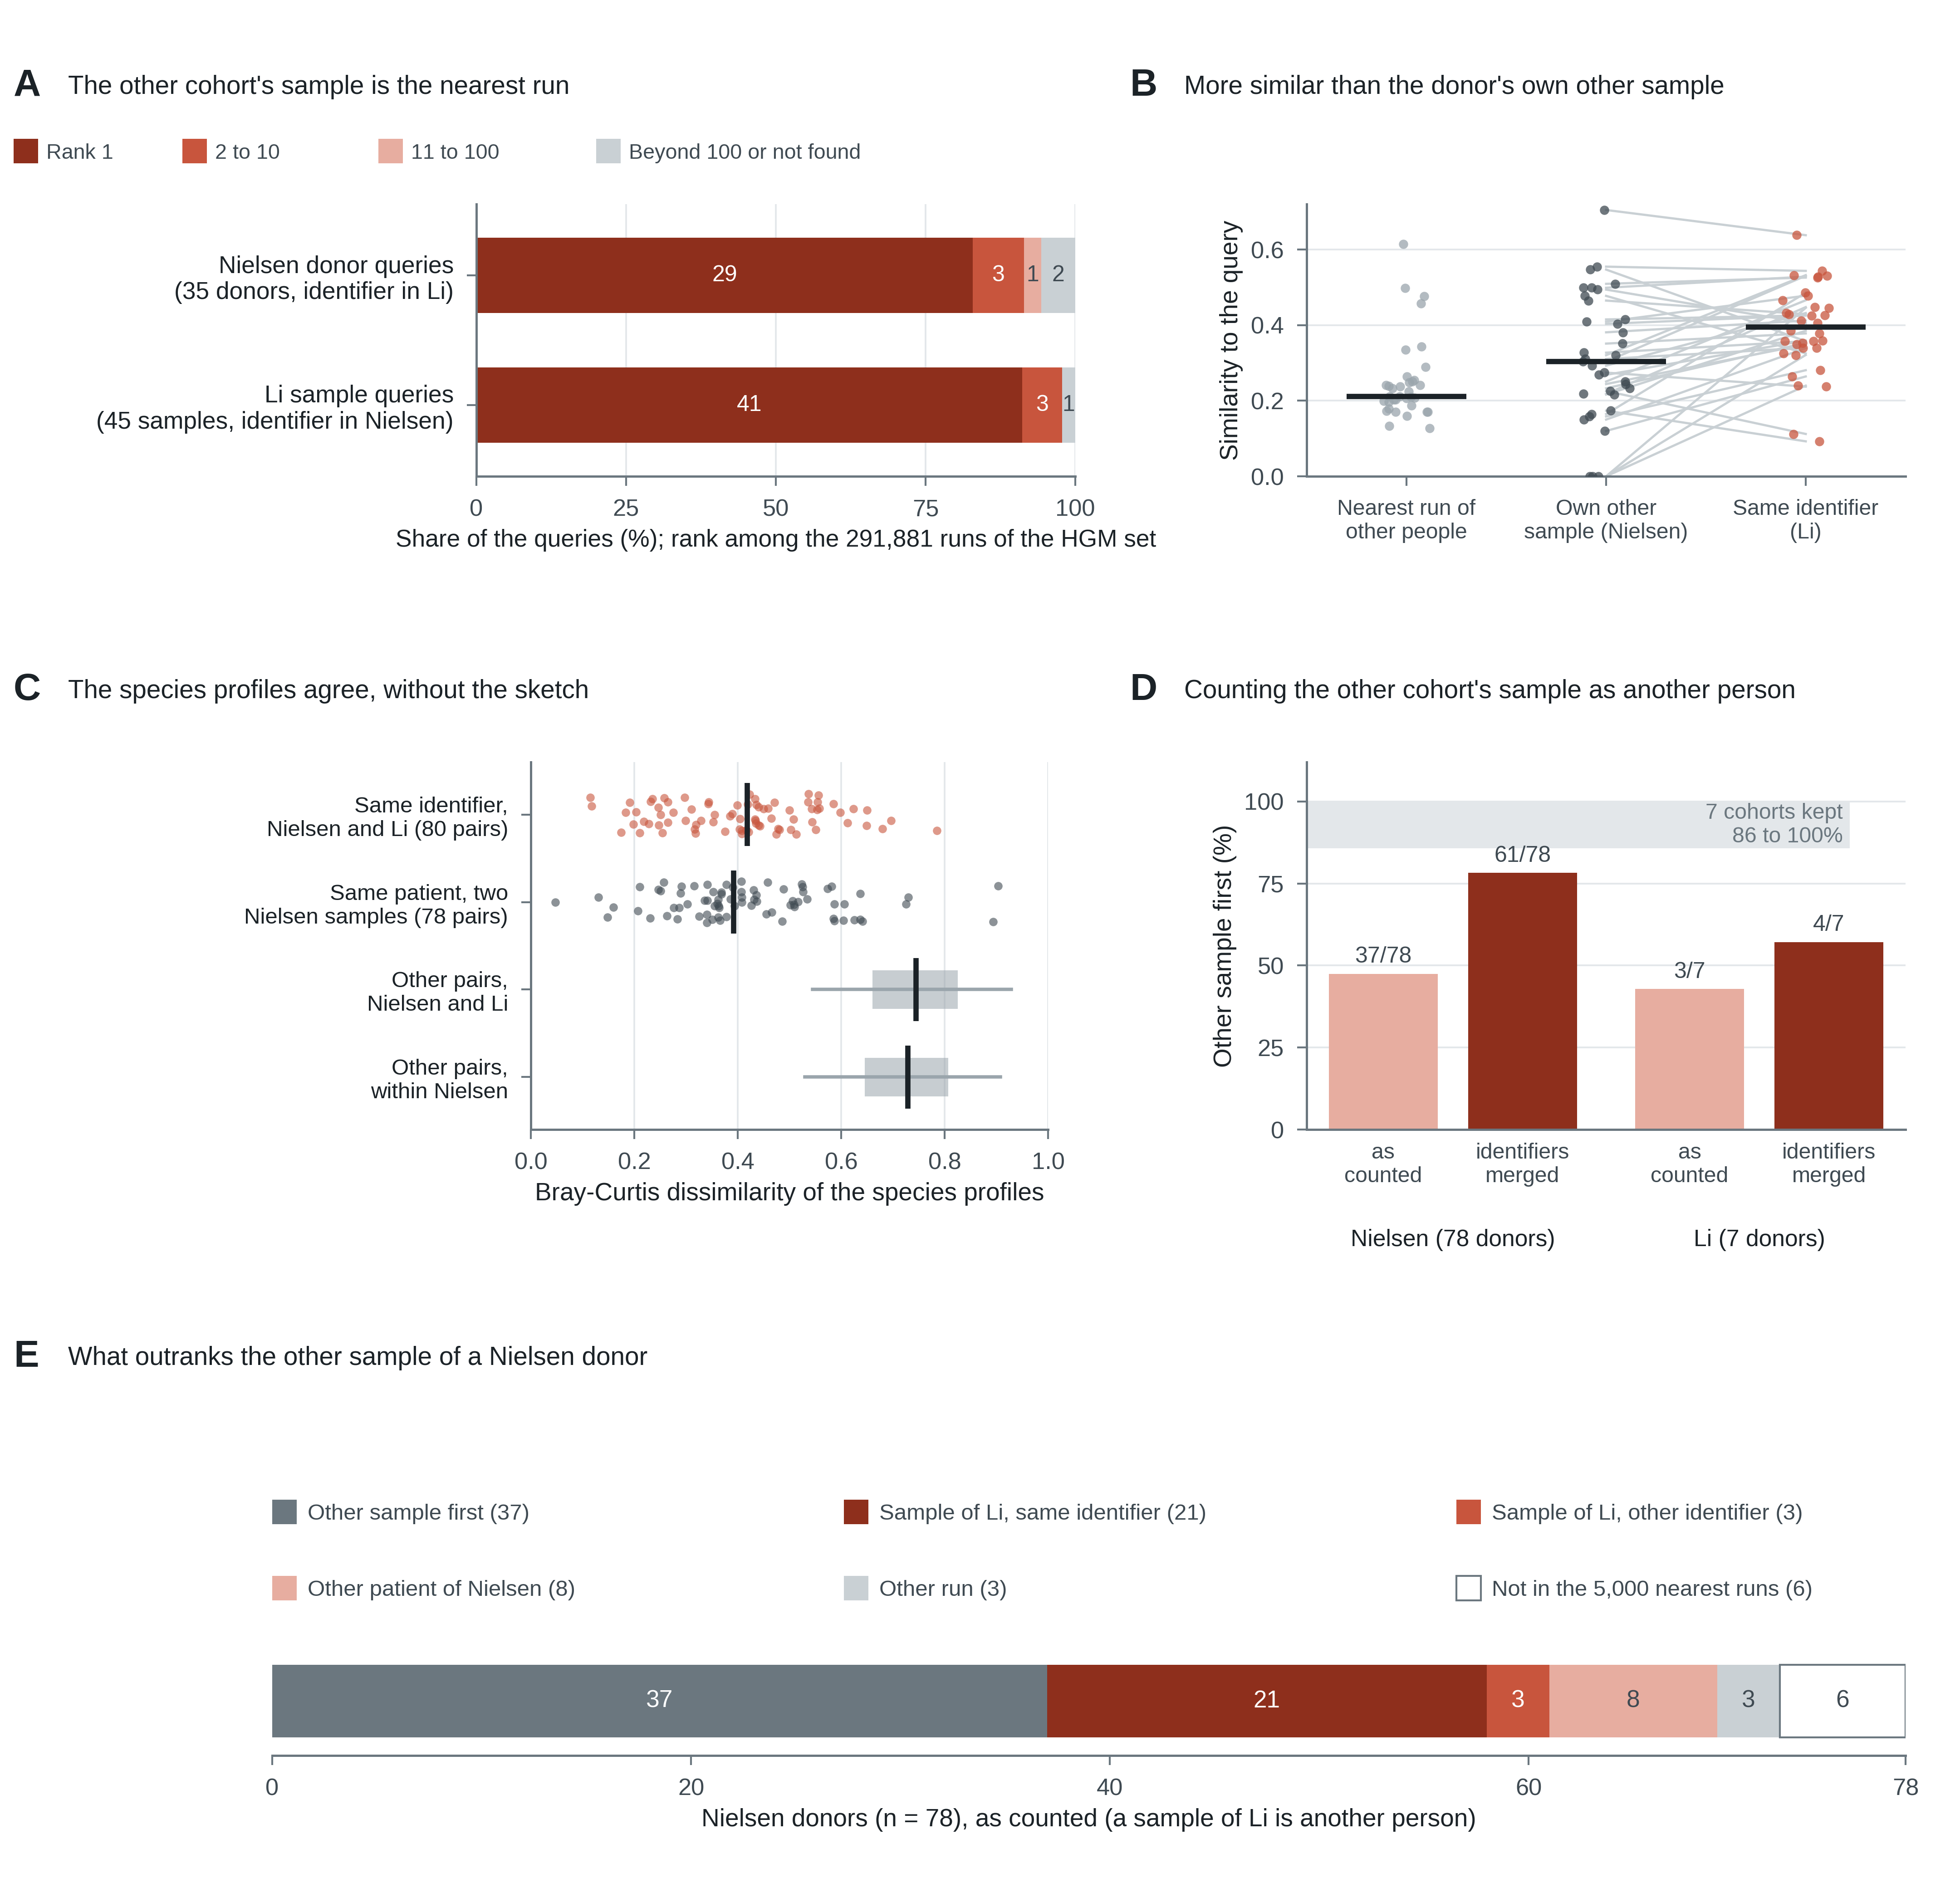
\includegraphics[width=\textwidth]{supplementary_figure2}
\caption[Links between the samples of Nielsen and Li]{\textbf{Links between the samples of Nielsen and Li.} \textbf{A}, Rank, among the 291,881 runs of the HGM set, of the most similar sample of the other cohort with the same subject identifier, when a donor of Nielsen queries the index (the 35 of the 78 Nielsen donors whose identifier has a sample in Li) and when a Li sample queries it (the 45 Li samples whose identifier has a sample in Nielsen); the other runs under that identifier, in either cohort, are not counted as runs of other people. \textbf{B}, Similarity to the query, for the 35 Nielsen donors of A, of the nearest run of other people among the runs of the HGM set (a sample of Li under the donor's identifier is not counted as another person here), of the donor's other sample in Nielsen and of the sample of the same identifier in Li (a line joins these last two samples of a donor when both are drawn; bar, median). For 3 donors the other sample is not among the 5,000 nearest runs, and it is drawn at 0 and enters the median as 0. The sample of Li is among the 5,000 nearest runs for 34 of the 35 donors, and only these 34 are drawn and enter the median. \textbf{C}, Bray-Curtis dissimilarity between species profiles, for a Nielsen and a Li sample with the same subject identifier (a dot per pair), two samples of one Nielsen patient (a dot per pair), and all the other pairs of a Nielsen and a Li sample and of two Nielsen samples (box, interquartile range; whiskers, 5th to 95th percentile). The bar is the median of each of the four groups. \textbf{D}, Share of the 78 Nielsen donors and of the 7 Li donors whose other sample is first among the 291,881 runs, when a sample of the other cohort under the donor's identifier counts as another person (as counted) and when it counts as the donor's own (identifiers merged); the band is the range of this share across the 7 cohorts kept. \textbf{E}, Outcome for the 78 Nielsen donors when Li samples count as other people: the other sample is first, another sample has higher similarity (classed by the nearest run of other people: a sample of Li with the donor's identifier, a sample of Li with another identifier, another patient of Nielsen or a run outside the two cohorts), or it is not among the 5,000 nearest runs.}
\end{figure}

The queried runs are paired runs of Genome Analyzer IIx instruments for the 78 Nielsen donors and of HiSeq 2000 instruments for the 7 Li donors (median 3.6 and 5.2 Gbp). Over the whole cohorts, the paired runs of Nielsen have a median of 68 bp per mate, compared with 82 bp for Li (Supplementary Table 6). The link thus holds across a change of instrument, read length and depth, against runs of other people that include those of the other patients of Nielsen.

\setcounter{table}{5}
\begin{table}[!htbp]\centering\small
\caption[Sequencing of the samples of Nielsen and Li]{\textbf{Sequencing of the samples of Nielsen and Li.} Run-level records of the ENA for the two projects, all stool samples of the two cohorts. \textit{Bases per mate}, the mean read length of a paired run, for the reads as deposited after the processing of the submitters.}
\begin{tabular}{>{\raggedright\arraybackslash}p{6.0cm}>{\raggedright\arraybackslash}p{4.5cm}>{\raggedright\arraybackslash}p{4.5cm}}
\toprule
 & Nielsen 2014 & Li 2014 \\
\midrule
ENA project & PRJEB1220 & PRJEB5224 \\
Runs; samples & 1,704; 396 & 579; 260 \\
Instrument of the paired runs & Genome Analyzer IIx (852 of 852) & HiSeq 2000 (287 of 287) \\
Instrument of all the runs & Genome Analyzer IIx 1,310, Genome Analyzer II 264, HiSeq 2000 130 & HiSeq 2000 579 \\
Bases per mate of the paired runs, median (5th to 95th percentile) & 68 (52--82) & 82 (79--85) \\
Gbp per sample, all runs, median (interquartile range) & 3.8 (2.2--4.2) & 5.6 (5.1--6.4) \\
Queried runs of the donors & 78 paired Genome Analyzer IIx runs, median 3.6 Gbp & 7 paired HiSeq 2000 runs, median 5.2 Gbp \\
Library names & 125 & 29 (0 in common) \\
Record created in the ENA & December 2012 & January and May 2014 \\
Centre label & BGI & Beijing Genome Institute; BGI \\
DNA extraction & Not recorded (none in the curated metadata) & Not recorded (MoBio kit in the curated metadata) \\
\bottomrule
\end{tabular}
\end{table}

\textbf{Resemblance between samples with the same identifier.} We looked for resemblance measured without the sketch (Supplementary Table 7). Species profiles find a Nielsen sample of the same identifier first among the 396 Nielsen samples for 32 of the 45 Li samples with the Bray-Curtis dissimilarity, 41 with the Aitchison distance and 42 with the Spearman correlation. They separate the pairs of a Nielsen and a Li sample of the same identifier from all the other pairs of a Nielsen and a Li sample with an area under the curve of 0.96, 0.997 and 0.98 (Supplementary Table 7; Supplementary Fig. 2C for the Bray-Curtis dissimilarity). The Bray-Curtis dissimilarity of a Nielsen and a Li sample of the same identifier (median 0.42) is close to that of two samples of one Nielsen patient (0.39) and below that of the samples of two Nielsen patients (0.73). The sex, age and body mass index recorded for the two cohorts agree (sex for 44 of 44 patients, age within one year for 41, body mass index within 0.5 kg per m$^2$ for 37), but the supplementary table of Li gives no clinical variable and the values curated for Li equal those of the published table of Nielsen.

\setcounter{table}{6}
\begin{table}[!htbp]\centering\footnotesize\setlength{\tabcolsep}{4pt}
\caption[Resemblance between the samples of Nielsen and Li with the same identifier]{\textbf{Resemblance between the samples of Nielsen and Li with the same identifier.} A pair is a Nielsen sample and a Li sample; the pairs of the same identifier are those of the 44 subject identifiers present in both cohorts. First means rank 1 among the 291,881 runs of the HGM set in the two lines on the sketch index, where the runs of the other samples of the same identifier are not counted as runs of other people, and among the 396 Nielsen samples in the three lines on species profiles. AUC, area under the curve of the dissimilarity for telling the pairs of the same identifier from the other pairs of Nielsen and Li.}
\begin{tabular}{>{\raggedright\arraybackslash}p{4.3cm}>{\raggedright\arraybackslash}p{6.4cm}>{\raggedright\arraybackslash}p{4.4cm}}
\toprule
Line of evidence & Result & Limit \\
\midrule
Sketch index, a Nielsen donor queries (35 donors) & Li sample of the same identifier first for 29 & Same labels and same index in both directions \\
Sketch index, a Li sample queries (45 samples) & Nielsen sample of the same identifier first for 41; both directions for 29 of 35 donors & Same labels and same index; deeper runs queried \\
Species profiles, Bray-Curtis & Nielsen sample first among 396 for 32 of 45; AUC 0.962 & Alike composition, not identity \\
Species profiles, Aitchison & First for 41 of 45; AUC 0.997 & As above; depends on a pseudocount \\
Species profiles, Spearman & First for 42 of 45; AUC 0.984 & As above \\
Bray-Curtis dissimilarity, median & 0.42 (same identifier, Nielsen and Li), 0.39 (two samples of one Nielsen patient), 0.73 (two Nielsen patients), 0.74 (other pairs of Nielsen and Li) & Same consortium and disease \\
CroCoDeEL on the species tables of the two cohorts together & 11 events between a Nielsen and a Li sample, 3 with the same identifier and 8 with different identifiers & Alike profiles; resemblance not limited to samples of one identifier \\
Curated sex, age, body mass index & Sex 44 of 44, age within one year 41, body mass index within 0.5 kg per m$^2$ 37 & The values of Li equal those of the published table of Nielsen \\
Run accessions, sample accessions or library names in common & None; highest similarity to a sample of the same identifier 0.67 & Reads not compared, so a re-deposit is not excluded \\
Host genotype, strain tracking, family & Not done; no family information in the metadata & Identity not confirmed \\
\bottomrule
\end{tabular}
\end{table}

We keep Nielsen and Li out of the main analysis for two reasons. (1) The links cannot be separated from the identifiers that define them (previous paragraph). (2) We can resolve the overlap of identifiers only in part (above), and the recovery rate of Nielsen depends on how the samples under a shared identifier are counted. Counting a Li sample under the donor's identifier as the donor's own, and no longer as another person's, raises the recovery rate of Nielsen from 47\% to 78\% (37 and 61 of 78 donors; Supplementary Fig. 2D,E).

\subsubsection*{Vincent}\addcontentsline{toc}{subsubsection}{Vincent}

Many samples of this cohort hold mostly human DNA. We measured human DNA for the 558 donors of the 7 cohorts kept and of Vincent (the 497 donors of the cohorts kept, before the two rules below, and the 61 donors of Vincent). The human share of a sample is the percentage of the hashes of its sketch that match a human genome, the sketch being recomputed from the public unitigs of the run (Methods). The human share of a donor is the higher of its two samples. It has a median of 48\% over the 61 donors of Vincent (up to 96\%), compared with 0.03\% over the 497 donors of the 7 cohorts kept. It is 5\% or more for 50 of the 61 donors of Vincent, compared with 13 of the 497 (Supplementary Fig. 3A). Over the 558 donors the share recovered falls as the human share rises. It is 93\% below 0.5\% human hashes (441 donors), 83\% from 0.5 to 5\% (54), 68\% from 5 to 50\% (34) and 14\% at 50\% or more (29; Supplementary Fig. 3B). We then removed the hashes that match a human genome and searched each query among the 1,116 runs (the two runs of each of the 558 donors). For the 495 donors under 5\%, the share whose other sample is the nearest of these runs does not change, 95\% before the removal and after it (Supplementary Fig. 3C). The removal restores part of the deficit of the 63 donors with 5\% or more. Their other sample is the nearest of the 1,116 runs for 32 of them before the removal and for 39 after. For the 61 donors of Vincent these counts are 27 before and 34 after, and 23 of the 61 are recovered in the HGM set. For 12 donors of Vincent one sample holds under 20\% human hashes and the other over 60\%, and 0 of them are recovered. The cohort was left out for its human content. Among the cohorts kept, 11 of the 13 donors with 5\% or more human hashes are recovered.

\setcounter{figure}{2}
\begin{figure}[!htbp]\centering
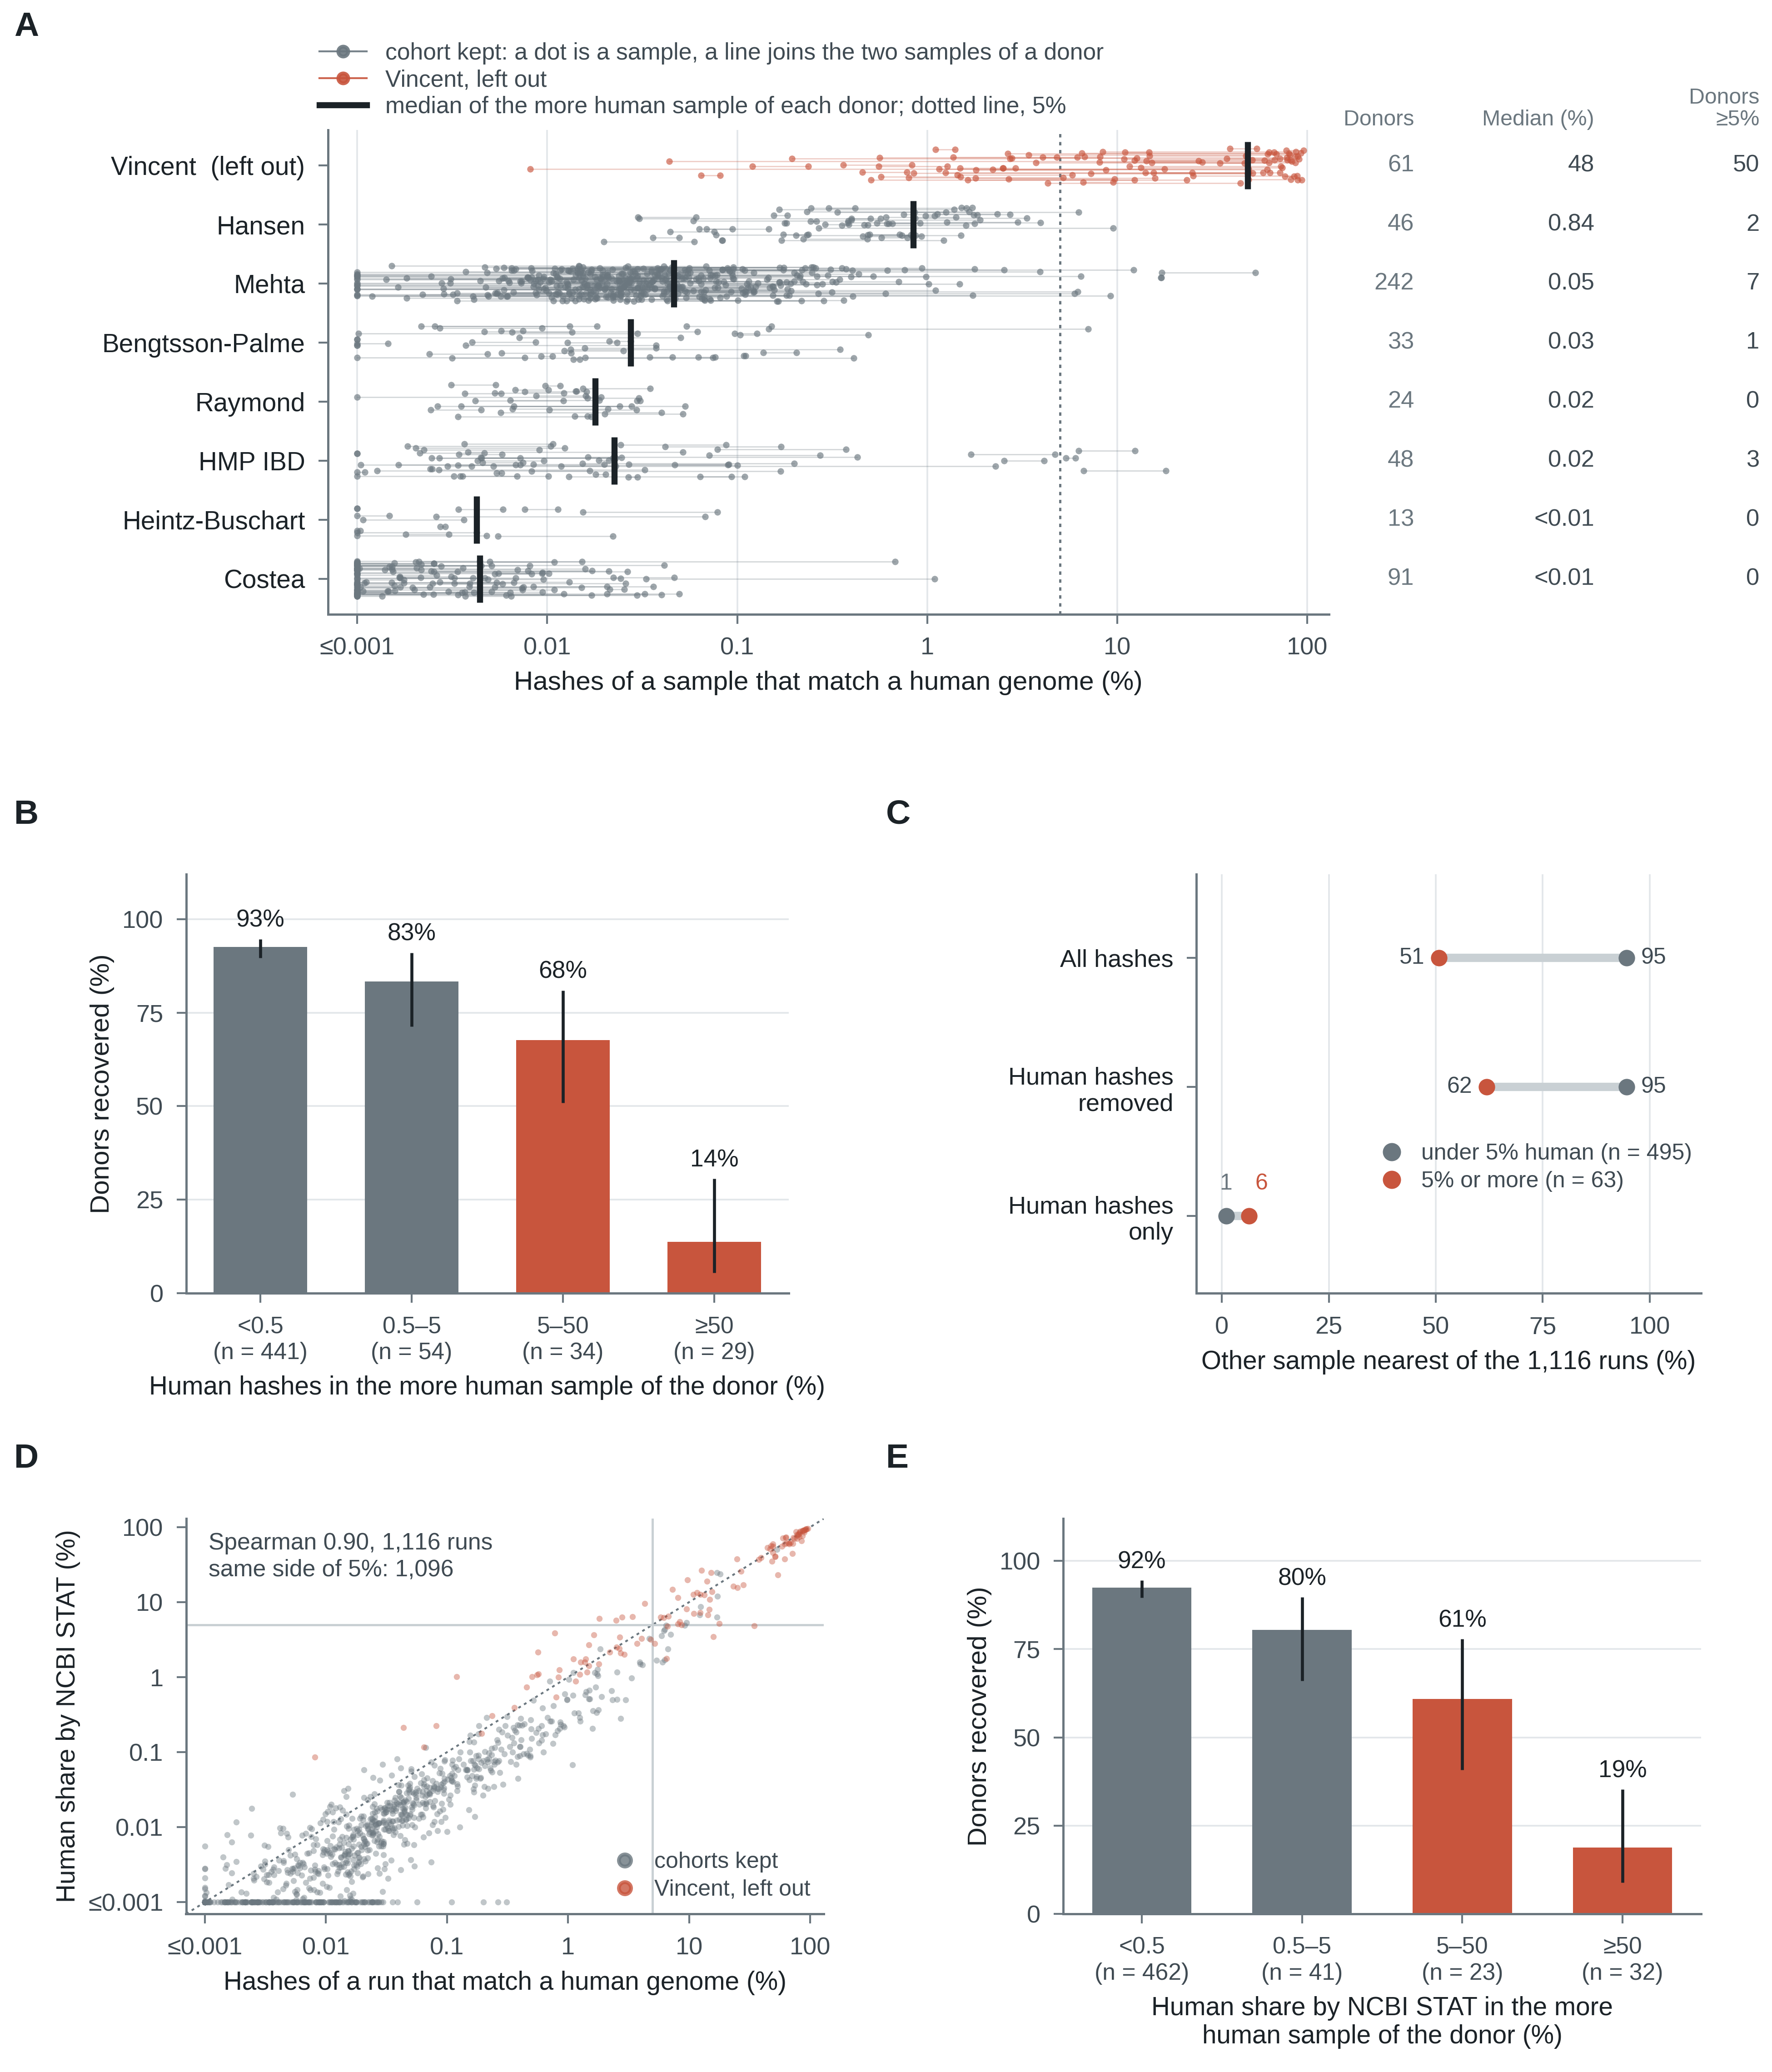
\includegraphics[width=\textwidth,height=0.71\textheight,keepaspectratio]{supplementary_figure3}
\caption[Human DNA in the samples of each cohort and share of donors recovered]{\textbf{Human DNA in the samples of each cohort and share of donors recovered.} \textbf{A}, Share of the hashes of the sketch of each sample that match a human genome (T2T-CHM13v2.0 or GRCh38.p14), for the 558 donors of 8 cohorts, namely the 7 cohorts kept and Vincent, which was left out (red). A dot is a sample and a thin line joins the two samples of a donor; the bar is the median, over the donors of the cohort, of the more human of their two samples; the dotted line marks 5\%; shares under 0.001\% are drawn at 0.001\%. \textbf{B}, Share of the 558 donors whose other sample is the nearest of the 291,881 runs of the HGM set, by the human share of the more human of their two samples (95\% Wilson intervals; the number of donors is under each bar; red, the two classes at 5\% or more). \textbf{C}, Share of donors whose other sample is the nearest of the 1,116 runs of the 558 donors (the two samples of each donor), with all hashes, without the hashes that match a human genome and with these hashes only, for the 495 donors whose more human sample holds under 5\% human hashes and the 63 donors with 5\% or more. The sketches were recomputed from the public unitigs of the runs (Methods). \textbf{D}, Share of the hashes of each of the 1,116 runs of C that match a human genome, against the human share of the same run in the NCBI taxonomic analysis (STAT; Supplementary Note 1), for the 7 cohorts kept (grey) and Vincent (red); the dotted line is the diagonal and the grey lines mark 5\%. \textbf{E}, As B, with the STAT human share.}
\end{figure}

\textbf{Independent estimate of the human share.} The NCBI runs a k-mer taxonomic analysis on every run of the SRA (STAT version 2.1.0\cite{katz2021}). We downloaded its result for the runs of the cohorts. The share of the species-level hits that STAT assigns to \textit{Homo sapiens} is a second human share of each run, computed on the run itself and not on our sketches. The two shares are correlated in rank (Spearman correlation 0.90 over the 1,116 runs, 0.93 over the 800 runs whose sketch holds 11 human hashes or more and 0.45 over the 316 others, whose share rests on 10 human hashes or fewer; Supplementary Fig. 3D). They place 1,096 of the 1,116 runs on the same side of 5\%, 83 at 5\% or more by both and 1,013 below 5\% by both (Cohen's $\kappa$ 0.88). Of the other 20 runs, 15 are at 5\% or more by the hashes only and 5 by STAT only. STAT gives a lower share than the hashes when human DNA is scarce and a close one when it is abundant. Vincent holds 80 of the 98 runs at 5\% or more by the hashes and 80 of the 88 by STAT, and no run of Costea, Raymond or Heintz-Buschart reaches 5\% by either measure (largest share in Costea 1.1\% by the hashes and 0.3\% by STAT). By donor, the more human of the two samples is at 5\% or more for 49 of the 61 donors of Vincent by STAT and for 50 by the hashes, and for 6 of the 497 donors of the cohorts kept by STAT and for 13 by the hashes. The share recovered falls with the STAT human share as it does with ours, 92\% below 0.5\% (462 donors), 80\% from 0.5 to 5\% (41), 61\% from 5 to 50\% (23) and 19\% at 50\% or more (32; Supplementary Fig. 3E). STAT is thus an independent indication, on another scale, that the human content is not an artefact of our references.

\subsection*{Rules of contamination and re-deposit}\addcontentsline{toc}{subsection}{Rules of contamination and re-deposit}

Two rules remove 14 of the 497 donors of the cohorts kept. The first removes the samples studied that take part, as source or target, in a CroCoDeEL event between two people at a rate above 5\% (below). It removes 9 samples, and 8 donors leave the analysis, 4 whose query sample is removed and 4 that have no other sample left. Of these 8 donors, 3 would have been recovered. The second removes the donors whose nearest run of other people has a similarity to the query above the highest similarity of the other sample of any donor that the first rule leaves. They are the six donors of Costea described below that the first rule leaves (the first rule removes the seventh). Their nearest run of other people carries the reads of their own sample under another subject code, and none of them was recovered. In HMP IBD, the public table of the consortium gives to its participants runs of two other projects of the consortium, PRJNA306874 and PRJNA389280. Such a run counts as the participant's own, neither its other sample nor a run of other people (618 runs of 88 participants, 41 of them donors of the analysis). This changes the rank of the other sample of no donor. It changes the rank of the first sample alone for 8 donors and that of the samples at least 30 days from the query for 1. It also removes the deposits of the donor's own samples from the search for an absent person (Fig. 1H).

\subsubsection*{Cross-sample contamination}\addcontentsline{toc}{subsubsection}{Cross-sample contamination}

We ran CroCoDeEL version 1.3.1 on the species table of each of 11 cohorts, the 7 kept and the 4 left out of the analysis (above), with all the samples of the cohort, the default settings of the tool and no abundance filter. We report only the events in which a sample studied takes part, as source or target. The samples studied are the query sample, the first sample and the most similar other sample of each donor (Supplementary Fig. 1B). They are 1,186 samples for the 497 donors of the cohorts kept, before the two rules above, and 391 for the 183 donors of the cohorts left out. The tool treats cross-sample contamination as a dilution, in which a source sample adds species to a target sample. These species keep in the target the relative abundances that they have in the source, multiplied by one constant, the rate. On log scales of source and target abundances, these species lie on a line of slope one, the contamination line. A random forest scores each pair that has a contamination line, and pairs with a probability of at least 0.5 are reported as events. Every pair of samples is tested in both directions, so it can give two events. An event is between two people when its two samples belong to different subjects of the curated metadata, and between two samples of one person otherwise. Indeed, CroCoDeEL can flag as contaminated two longitudinal samples of one individual, especially over short intervals, among the causes of false positives\cite{goulet2026} (README of the tool).

Events between two people are few among the samples studied of the cohorts kept (Supplementary Fig. 4 and Supplementary Table 8). These 1,186 samples take part in 277 events, 10 of them (4\%) between two people. Of the 1,186 samples, 10 (0.8\%) take part in at least one of the 10 events between two people, from none of the samples studied of Heintz-Buschart and Raymond to 6.1\% of those of Bengtsson-Palme (4 of 66). The rate of these 10 events has a median of 78\% (range 3\% to 90\%). In Pehrsson, all 71 events in which a sample studied takes part are between two people, and 55 of its 83 samples studied (66\%) take part in at least one of these 71 events (above). In Nielsen, Li and Vincent, also left out, 15 of 156, 0 of 16 and 4 of 136 samples studied take part in at least one event between two people (9.6\%, 0.0\% and 2.9\%), compared with none to 6.1\% in the cohorts kept.

\setcounter{figure}{3}
\begin{figure}[!htbp]\centering
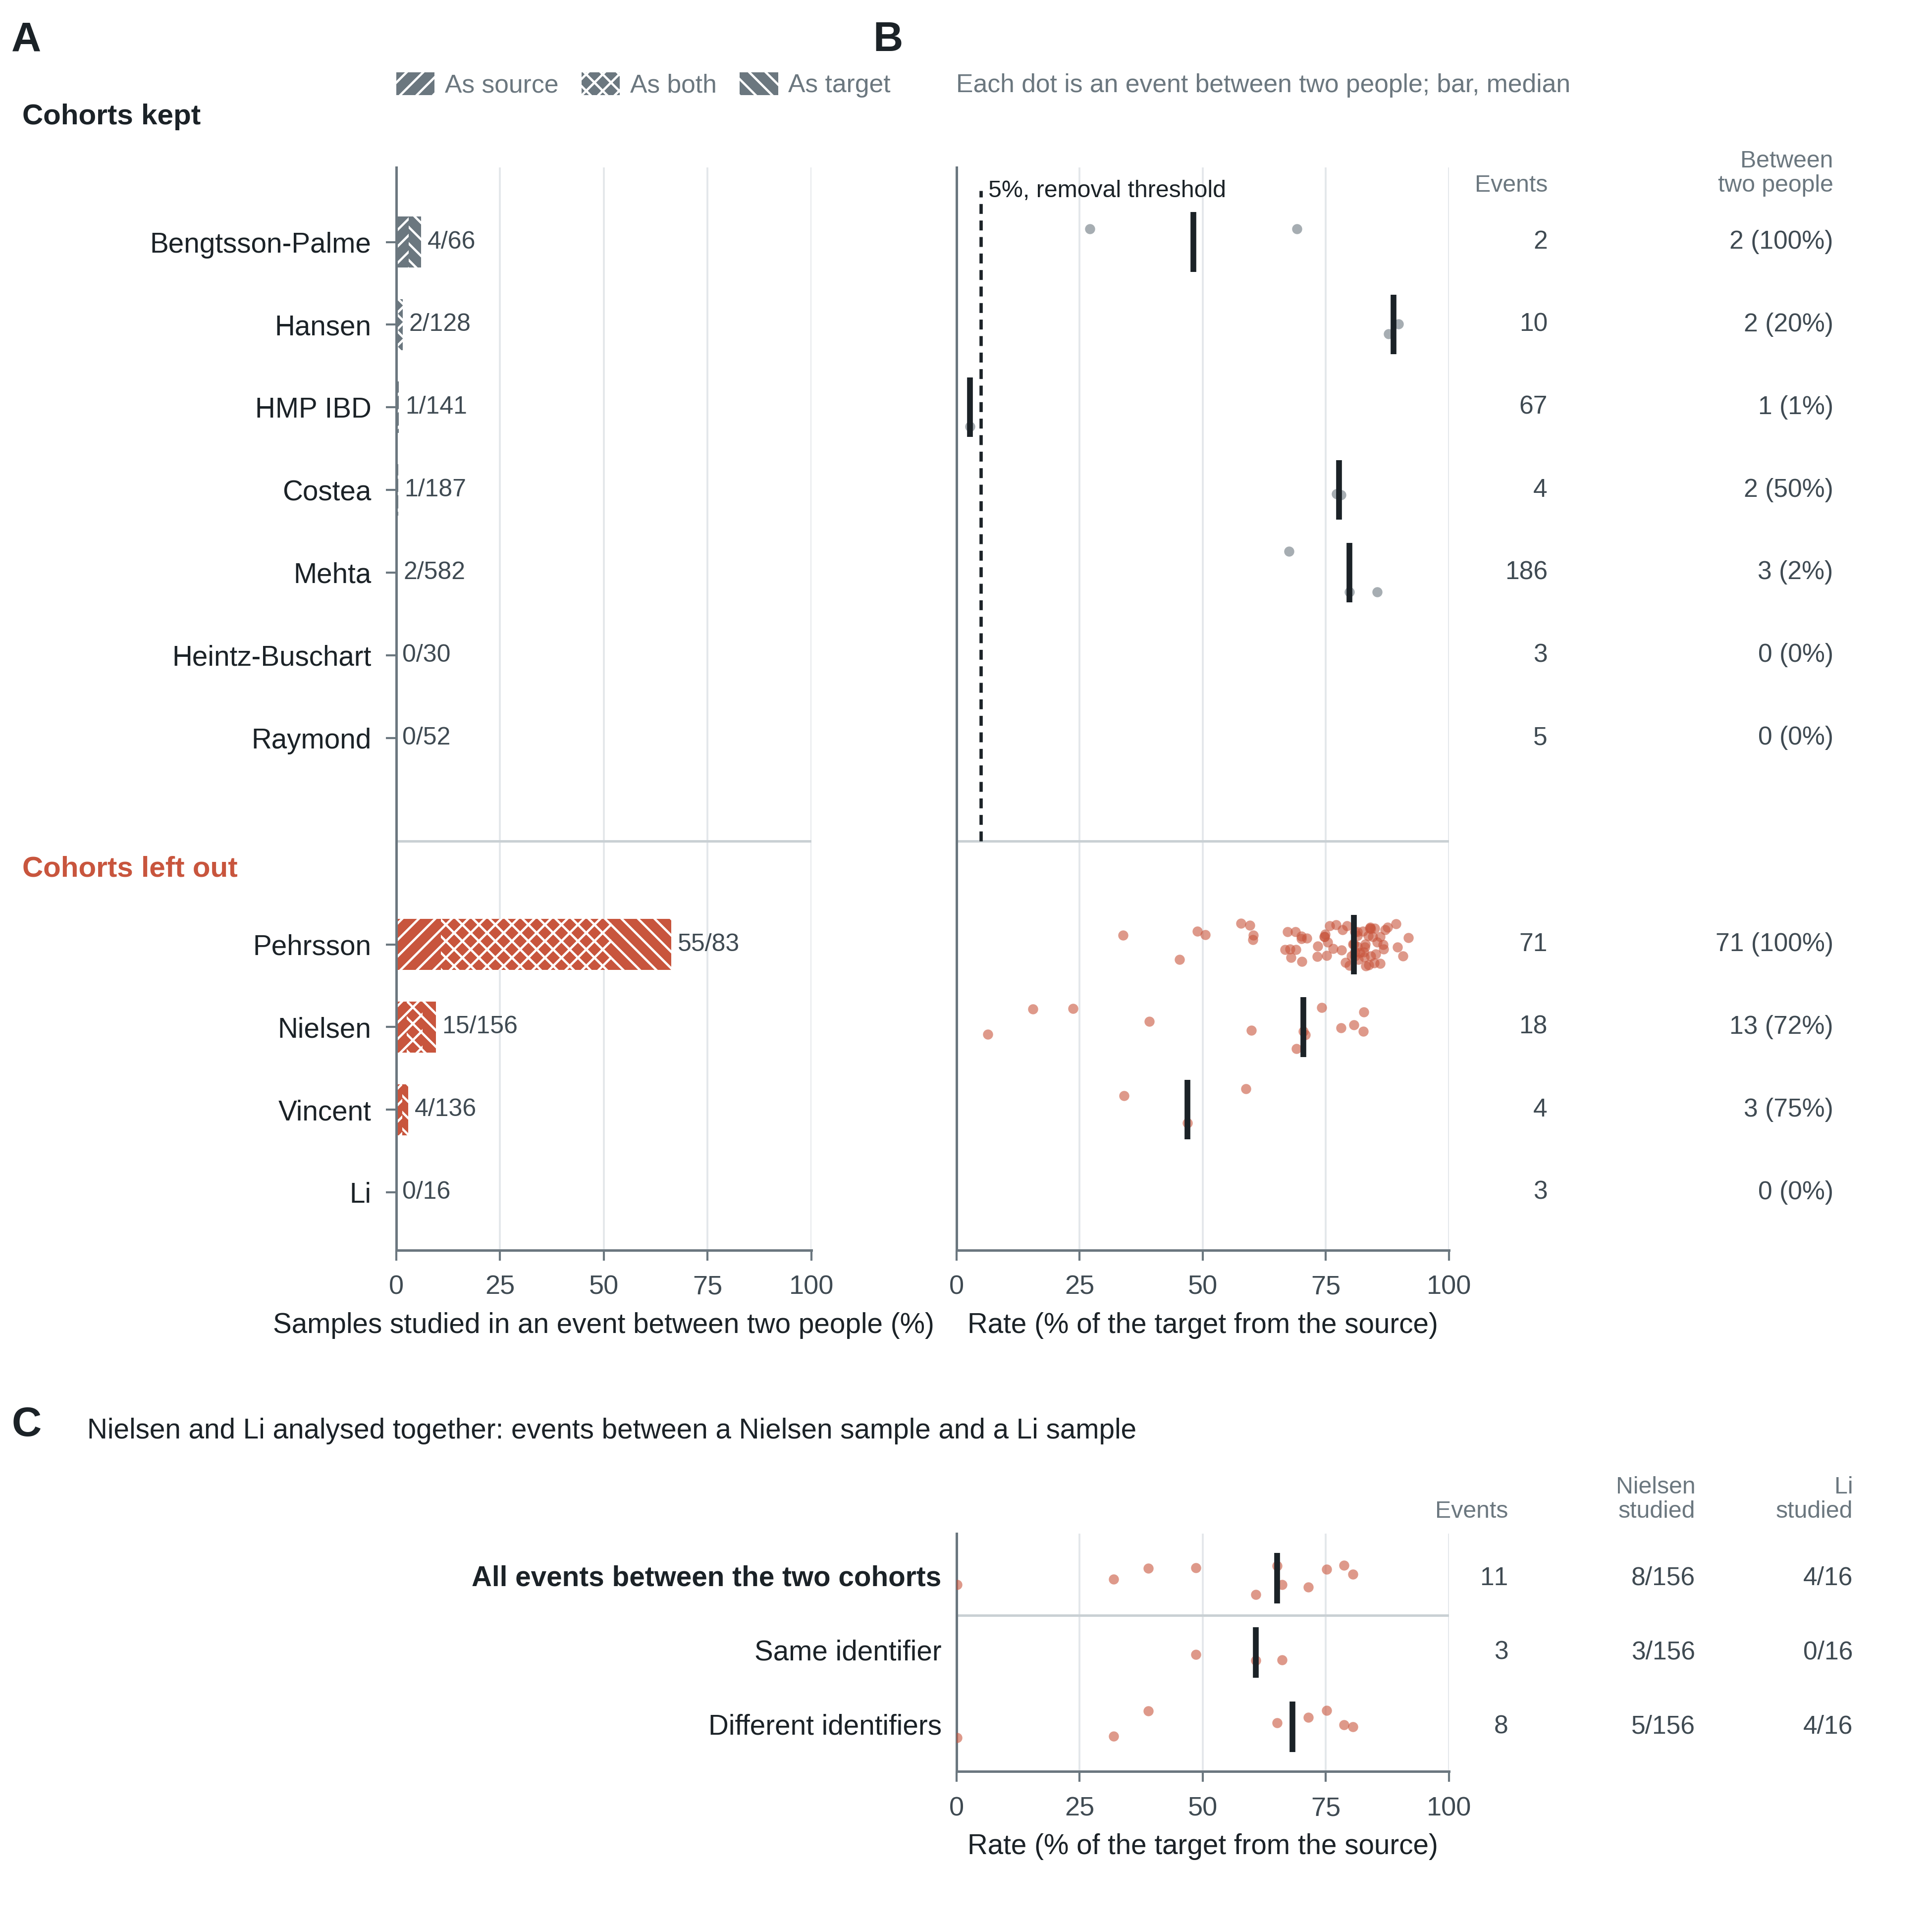
\includegraphics[width=\textwidth]{supplementary_figure4}
\caption[CroCoDeEL events between two people, by cohort]{\textbf{CroCoDeEL events between two people, by cohort.} Events in which a sample studied takes part, as source or target, in the 7 cohorts kept (grey) and the 4 cohorts left out of the analysis (red). The samples studied are the query sample, the first sample and the most similar other sample of each donor, in the cohorts kept those of the 497 donors before the two rules of Supplementary Note 1. CroCoDeEL was run on the species table of each cohort, with all its samples. Each event that the tool reports has a source sample and a target sample in the same species table (Supplementary Note 1), and it is between two people when its two samples belong to different subjects of the curated metadata. \textbf{A}, Share of the samples studied of each cohort that take part in at least one event between two people (samples concerned over samples studied), hatched according to whether the sample is a source (right-leaning), a target (left-leaning), or both (cross-hatched). \textbf{B}, Rate of each of these events, the share of the target that comes from the source, in percent (a dot per event, the bar is the median), with the number of events in which a sample studied takes part and the number of them between two people. Dashed line, 5\%, the rate above which the rule of contamination of Supplementary Note 1 removes the samples studied of an event between two people in the cohorts kept. Cohorts are ordered by the share in A within each group. \textbf{C}, Nielsen and Li carry the same subject identifiers for 44 patients, so CroCoDeEL was also run on their two species tables merged, and the panel shows the events between a Nielsen sample and a Li sample in which a sample studied takes part, all together and by whether the two samples carry the same subject identifier (a dot per event, the bar is the median), with the number of events and the number of samples studied of each cohort that take part in one.}
\end{figure}

\setcounter{table}{7}
\begin{table}[!htbp]\centering\small
\caption[Events between two people, by cohort]{\textbf{Events between two people, by cohort.} CroCoDeEL events in which a sample studied takes part, as source or target, in each of the 11 cohorts (the 7 kept and the 4 left out); Supplementary Fig. 4 draws them. \textit{Samples}, samples of the cohort in the curated tables and, in parentheses, the samples studied, namely the query sample, the first sample and the most similar other sample of each donor, in the cohorts kept those of the 497 donors before the two rules of Supplementary Note 1. \textit{Events}, events in which a sample studied takes part. \textit{Between two people}, number of these events whose two samples belong to different subjects of the curated metadata, and share of the events (\%). \textit{In such an event}, samples studied that take part in at least one event between two people, and share of the samples studied (\%). \textit{Rate}, median and range of the rate of the events between two people, the share of the target that comes from the source, in percent.}
\setlength{\tabcolsep}{5pt}
\begin{tabular}{lrrrrr}
\toprule
Cohort & Samples (studied) & Events & Between two people & In such an event & Rate (\%) \\
\midrule
\multicolumn{6}{l}{\textit{Cohorts kept}} \\
Bengtsson-Palme & 70 (66) & 2 & 2 (100) & 4 (6.1) & 48 (27--69) \\
Hansen & 207 (128) & 10 & 2 (20) & 2 (1.6) & 89 (88--90) \\
HMP IBD & 1,627 (141) & 67 & 1 (1) & 1 (0.7) & 3 (3--3) \\
Costea & 279 (187) & 4 & 2 (50) & 1 (0.5) & 78 (77--78) \\
Mehta & 928 (582) & 186 & 3 (2) & 2 (0.3) & 80 (68--85) \\
Heintz-Buschart & 53 (30) & 3 & 0 (0) & 0 (0.0) & -- \\
Raymond & 72 (52) & 5 & 0 (0) & 0 (0.0) & -- \\
\midrule
All cohorts kept & 3,236 (1,186) & 277 & 10 (4) & 10 (0.8) & 78 (3--90) \\
\midrule
\multicolumn{6}{l}{\textit{Cohorts left out}} \\
Pehrsson & 191 (83) & 71 & 71 (100) & 55 (66.3) & 81 (34--92) \\
Nielsen & 396 (156) & 18 & 13 (72) & 15 (9.6) & 70 (6--83) \\
Vincent & 229 (136) & 4 & 3 (75) & 4 (2.9) & 47 (34--59) \\
Li & 260 (16) & 3 & 0 (0) & 0 (0.0) & -- \\
\midrule
All cohorts left out & 1,076 (391) & 96 & 87 (91) & 74 (18.9) & 79 (6--92) \\
\bottomrule
\end{tabular}
\end{table}

Nielsen and Li carry the same subject identifiers for 44 patients (above), so we also ran CroCoDeEL on their two species tables merged (656 samples; Supplementary Fig. 4C) to find events between the two cohorts. The tool reports 11 events between a Nielsen and a Li sample, and a sample studied takes part in each of them. Their median rate is 65\% (range 0.1\% to 81\%). These 11 events join 9 pairs of samples. Of the 156 Nielsen samples studied, 8 take part in at least one of them, as do 4 of the 16 Li samples studied. Three of these events join two samples that carry the same subject identifier (rates 49\% to 66\%) and 8 join samples with different identifiers (median rate 68\%). The 8 Nielsen samples studied that take part in these 11 events belong to 6 donors, too few to account for the 41 Nielsen donors that are not recovered.

The 10 samples studied of the cohorts kept that take part in an event between two people belong to 9 donors. The query sample is one of them for 4 donors, in events at rates of 77\% to 90\%, and none of these donors is recovered. Another sample studied is one of them for 5 donors, in events at rates of 3\% to 69\%. The rule of contamination removes the samples in such an event at a rate above 5\%, so 8 of these donors leave the analysis. The last, a donor of HMP IBD, keeps its most similar other sample, which takes part in an event at 2.8\%, and stays in the analysis.

Contamination between samples of a cohort, as CroCoDeEL detects it, does not account for the recoveries of the 483 donors of the analysis. The query sample took part in no event for 370 of the 483 donors, and 92.4\% of these 370 donors are recovered in the HGM set, compared with 94.0\% of all 483 donors. The 30-day subset (Methods) holds the 354 donors with another sample at least 30 days from the query, and the most similar of those samples takes the place of their other sample. The query sample took part in no event for 295 of these 354 donors, and 93.2\% of these 295 donors are recovered, compared with 94.1\% of all 354.

\subsubsection*{Reads of seven Costea donors deposited under another subject code}\addcontentsline{toc}{subsubsection}{Reads of seven Costea donors deposited under another subject code}

For 7 of the 497 donors of the cohorts kept the nearest run of other people has a similarity of 0.78 to 0.89. Among the 490 other donors its highest similarity is 0.49. The seven similarities are also higher than the highest similarity of the other sample of any donor, which is 0.65. The seven are the 7 donors of Costea with a German subject identifier. None of them is recovered, and they make up 7 of the 19 donors of the cohort that are not recovered. For each of the seven we looked up the nearest run of other people, which we call the matched run, in the public records of the ENA and of BioSamples. We then compared its reads with those of the queried run. Supplementary Table 9 gives the results donor by donor.

\setcounter{table}{8}
\begin{table}[!htbp]\centering\footnotesize\setlength{\tabcolsep}{2.5pt}
\caption[Queried and matched runs of the seven Costea donors]{\textbf{Queried and matched runs of the seven Costea donors.} \textit{Donor}, subject identifier of curatedMetagenomicData; the reproduction package gives the runs of each donor. \textit{Days}, between the first and the last sample of the donor. \textit{Other sample}, its similarity to the query and its rank among the 291,881 runs of the HGM set, before the removal of the seven donors (Supplementary Note 1). \textit{Match}, similarity of the nearest run of other people, a run of PRJEB41102. \textit{Reads}, read 1 of the queried run on the first tile of the flow cell. \textit{Found}, share of these reads (\%) with a read at the same position (instrument, lane, tile, x, y) in the matched run. \textit{Day}, day of the query sample in the series of its donor, as given by its Costea name; PRJEB50977 holds a sample whose name gives that day and the subject code of the matched run. \textit{Gap}, days between the collection dates of the query sample and of that sample of PRJEB50977. \textit{Day} is counted from day 0 of the series, so it exceeds \textit{Days} for the one donor whose first curated sample is later. \textit{Sex}, record of the matched sample against the curated metadata (n.r., not recorded). \textit{Above}, number of runs of the HGM set that the pipeline counts as another person's and that are more similar than the donor's other sample and, in parentheses, how many of them carry the subject code of the matched run or are runs of PRJEB24041 whose sample name gives the same person as the Costea name of the query sample (the runs of one sample labelled with another subject code are counted under the subject code of the matched run; Supplementary Note 1). \textit{Rank}, rank of the other sample without those runs. --, the other sample lies beyond the 5,000 nearest runs.}
\begin{tabular}{lrlrrrrrlrr}
\toprule
Donor & Days & Other sample & Match & Reads & Found & Day & Gap & Sex & Above & Rank \\
\midrule
DEU1 & 41 & 0.44, rank 13 & 0.89 & 48,917 & 98.6 & 918 & 2 & Same & 12 (12) & 1 \\
DEU7 & 30 & Not in 5,000 & 0.79 & 92,897 & 100.0 & 30 & 0 & Same & -- & -- \\
DEU8 & 30 & 0.31, rank 24 & 0.78 & 71,319 & 100.0 & 30 & 0 & Same & 23 (23) & 1 \\
DEU13 & 30 & 0.36, rank 6 & 0.78 & 76,245 & 100.0 & 30 & 0 & Same & 5 (5) & 1 \\
DEU14 & 30 & 0.37, rank 10 & 0.78 & 18,270 & 100.0 & 30 & 0 & Same & 9 (9) & 1 \\
DEU18 & 918 & 0.42, rank 9 & 0.83 & 49,988 & 99.5 & 918 & 0 & Same & 8 (8) & 1 \\
DEU22 & 30 & 0.37, rank 15 & 0.81 & 86,089 & 100.0 & 30 & 0 & n.r. & 14 (14) & 1 \\
\bottomrule
\end{tabular}
\end{table}

For all seven, the matched run belongs to one project of the ENA, PRJEB41102, first public in November 2020, on strain persistence in the adults and infants of families. The queried runs belong to PRJEB17632, the project of Costea, and the same centre (EMBL) deposited both. PRJEB41102 records the matched sample under a subject code of its own. The curated metadata contain no link between the two projects, so the pipeline could have counted the matched run as belonging to another person.

We compared read 1 of the two runs on the first tile of the flow cell, from the public FASTQ files (18,270 to 92,897 queried reads per pair). In all seven pairs the two runs share the instrument, lane and tile. In each pair, 98.6\% or more of the queried reads have a read at the same position on the tile (same x and y coordinates) in the matched run (1 to 677 queried reads per pair have none). Over the seven pairs this makes 442,730 reads found in both runs. For every one of them the queried read is a strictly shorter part of the matched read (none is identical, none is longer). For 442,729 of the 442,730 this part has the same quality string in the two runs. The matched reads all have 94 bases, the queried reads 45 to 93. In every read found in both runs, the queried run lacks the first bases of the matched read (a median of 1 to 4 bases depending on the pair). In 10 to 19\% of these reads the queried run also lacks a tail (a median of 14 to 21 bases depending on the pair). On the tile the matched run holds 1.1 to 1.4 times as many reads as the queried run. The queried run is thus a trimmed and filtered version of the reads of the matched run. Each queried run also has an exact re-deposit in a third project of the same centre (PRJEB24041), a run with the same number of bases that has a similarity of 0.99 or more, and the pipeline removed it (Methods). These comparisons use the scripts \texttt{costea\_reads\_compare.py} and \texttt{costea\_trim\_filter.py} of the reproduction package.

The subject code of the matched run also names samples in a fourth project of the same centre (PRJEB50977, first public in October 2023), whose sample names give the day of the sample. For all seven, this project holds a sample of the code on the day given in the Costea name of the query sample (day 30 or 918). It also holds a sample of the code on all the other sampling days of the donor's curated series (3 to 8 sampling days per donor in all). The PRJEB50977 sample of the queried day has the collection date of the query sample, or a date 2 days away for 1 donor. The record of the matched sample gives the collection year of the query sample, the same sex as the curated metadata (not recorded for 1 donor) and an age within one year of the curated age plus the time from day 0 of the series to the query sample.

Six of the seven donors have their other sample among the 5,000 nearest runs. For each of them we looked at every run of the HGM set that the pipeline counts as another person's and that is more similar to the query than the other sample (5 to 23 runs per donor). Each of these runs either carries the subject code of the matched run or is a run of PRJEB24041, with a similarity below 0.99, whose sample name gives the same person as the Costea name of the query sample. For one of the six, 4 of these runs belong to a sample of PRJEB41102 labelled with another subject code. The record of this sample (sex, age, family role) is that of the subject code of the matched run, and its sample number is consecutive with those of that code. We therefore count these 4 runs under the subject code of the matched run. With all the runs above the other sample counted as the donor's own, the other sample would rank first for each of the six donors. The number of donors recovered would then rise from 72 of 91 (79\%) to 78 of 91 (86\%) in Costea and, over all the donors of the cohorts kept, from 457 of 497 (92.0\%) to 463 of 497 (93.2\%). The seventh donor would still not be recovered. In the open-set test of the 497 donors of the cohorts kept, the search for an absent person was accepted for all seven.

The seven are removed from the analysis (above), six by the rule of re-deposit and the one whose query sample takes part in a contamination event by the rule of contamination. We cannot list the runs of a person that sit in other projects under other identifiers, so other donors may have such runs at lower similarities, which the pipeline counts as other people. This could possibly explain why the Costea cohort has a lower recovery rate than the other cohorts (see below).

\FloatBarrier
\section*{Supplementary Note 2. Donors recovered and not recovered}\addcontentsline{toc}{section}{Supplementary Note 2. Donors recovered and not recovered}

Most donors are recovered, but not all. This Note looks at the donors that are not recovered, and at how the recovery rate varies between cohorts, with the time between the samples and with the depth of the query.

A donor is recovered when its other sample is at rank 1 (Methods). This is the case for 454 of 483 donors (94.0\%). The ranking is made among the 291,881 human gut metagenomes of the HGM set, which are part of the 4,791,208 runs of the index. The other 29 donors fall into two groups (Supplementary Fig. 1B and Supplementary Table 10). For 15 donors (3.1\%) the other sample is not among the runs that the Faure \textit{et al.} service returns. The service returns at most the 5,000 nearest runs, down to a similarity of 0.05, so these donors count as not recovered. For 14 donors (2.9\%) the other sample is returned, but at least one sample of another person has higher similarity to the query, placing the other sample at a median rank of 92.

\setcounter{table}{9}
\begin{table}[!htbp]\centering\footnotesize\setlength{\tabcolsep}{2.2pt}
\caption[Donors by rank of the other sample]{\textbf{Donors by rank of the other sample.} \textit{Rank 2 or more}, the other sample is among the 5,000 nearest runs returned, but at least one sample of another person has higher similarity to the query. \textit{Not in 5,000}, it is not among the 5,000 nearest runs returned by the Faure \textit{et al.} service. Similarities are medians of the similarities returned by the Faure \textit{et al.} service, with the interquartile range (IQR) in parentheses; the nearest run of other people is the most similar run of the whole index that is not assigned to the donor. We assigned runs to subjects only in the 12 adult cohorts that have donors in the index (Supplementary Table 2). Number of donors whose nearest run of other people is assigned to another subject of the donor's cohort (\textit{Same cohort}), to a subject of another of these 12 cohorts (\textit{Other cohort}) or to no subject of these 12 cohorts (\textit{Outside the 12}).}
\begin{tabular}{lrrrrrrr}
\toprule
 & & & \multicolumn{2}{c}{Median similarity (IQR)} & \multicolumn{3}{c}{Nearest run of other people from} \\
\cmidrule(lr){4-5}\cmidrule(lr){6-8}
 & Donors & \% of 483 & Other sample & Other people & Same cohort & Other cohort & Outside the 12 \\
\midrule
Recovered (rank 1) & 454 & 94.0 & 0.37 (0.32--0.42) & 0.19 (0.17--0.21) & 69 & 13 & 372 \\
Rank 2 or more & 14 & 2.9 & 0.14 (0.10--0.17) & 0.17 (0.15--0.18) & 5 & 0 & 9 \\
Not in 5,000 & 15 & 3.1 & -- & 0.17 (0.15--0.18) & 5 & 0 & 10 \\
\bottomrule
\end{tabular}
\end{table}

For the 14 donors whose other sample is at rank 2 or more, the other sample is far less similar to the query than for the 454 recovered donors (median similarity 0.14 compared with 0.37). For each donor we also took the nearest run of other people among all the runs of the index. Its median similarity to the query is 0.17 for the donors at rank 2 or more and 0.19 for the recovered donors (two-sided Mann--Whitney test, \textit{U} = 2,134, \textit{P} = 0.04). 

For the 15 donors whose other sample is not returned, the nearest run of other people has a median similarity of 0.17. The nearest run of other people comes from the donor's own cohort for 5 of the 14 donors at rank 2 or more (36\%), compared with 69 of the 454 recovered donors (15\%). For 9 of these 14 donors it is a run outside the 12 adult cohorts whose runs we resolved (Supplementary Note 1). Such a run counts as another person, which can only lower the recovery rate. When the nearest run of other people comes from the donor's cohort, it can be a run of a relative or of a cohabitant. It can also be a run of the donor curated under a second identifier or deposited under the label of another sample.
In the open-set test of Fig. 1H (Methods), 59 of the 483 searches for an absent person are accepted at its threshold. In 16 of these 59 searches (27\%) the nearest run of other people comes from the donor's own cohort, compared with 63 of the 424 searches that are not accepted (15\%).

The recovery rate differs between cohorts (Fig. 1D and Supplementary Table 11). Costea has the lowest rate, with 72 of its 84 donors recovered (86\%), whereas 95--100\% of the donors are recovered in each of the other 6 cohorts. To study the time between the samples, the first sample takes the place of the other sample (Fig. 1E and Supplementary Table 12). The first sample is at rank 1 in the HGM set for 91--93\% of the donors whose first sample is up to 180 days from the query, and for 81\% at 181--391 days.

\setcounter{table}{10}
\begin{table}[!htbp]\centering\footnotesize\setlength{\tabcolsep}{4pt}
\caption[Cohorts, ordered by the share of donors recovered]{\textbf{Cohorts, ordered by the share of donors recovered.} Cohorts are named by their curatedMetagenomicData identifiers. \textit{Recovered}, donors whose other sample is at rank 1 in the HGM set, the measure of Fig. 1D (also at rank 1 among all the runs of the index). \textit{Not in 5,000}, donors whose other sample is not among the 5,000 nearest runs returned, counted as not recovered. \textit{Interval}, median number of days between the query and the first sample, with the interquartile range (IQR) in parentheses. \textit{Query run}, median number of bases of the queried run in the ENA, in Gbp, with the IQR in parentheses. \textit{Runs}, median number of runs that the curated metadata list for the query sample (-- for HMP\_2019\_ibdmdb, whose curated metadata list none, and for all cohorts together; Supplementary Note 1).}
\begin{tabular}{lrrrrrr}
\toprule
Cohort & Donors & Recovered (\%) & Not in 5,000 & Interval (days) & Query run (Gbp) & Runs \\
\midrule
CosteaPI\_2017 & 84 & 72 (86) & 6 & 90 (90--90) & 1.4 (1.2--1.6) & 8 \\
MehtaRS\_2018 & 241 & 228 (95) & 6 & 2 (0--180) & 2.2 (1.7--2.6) & 1 \\
HansenLBS\_2018 & 44 & 42 (95) & 2 & 164 (154--180) & 6.7 (5.3--8.6) & 1 \\
RaymondF\_2016 & 24 & 23 (96) & 0 & 90 (90--90) & 0.81 (0.81--0.81) & 21 \\
HMP\_2019\_ibdmdb & 48 & 47 (98) & 1 & 268 (231--321) & 1.9 (1.7--2.3) & -- \\
Heitz-BuschartA\_2016 & 13 & 13 (100) & 0 & 56 (33--62) & 3.9 (3.8--4.0) & 1 \\
Bengtsson-PalmeJ\_2015 & 29 & 29 (100) & 0 & 72 (64--97) & 18 (15--21) & 1 \\
\midrule
All cohorts & 483 & 454 (94) & 15 & 90 (2--180) & 2.1 (1.4--3.0) & -- \\
\bottomrule
\end{tabular}
\end{table}

\setcounter{table}{11}
\begin{table}[!htbp]\centering\small
\caption[Interval between the query and the first sample]{\textbf{Interval between the query and the first sample.} The query is the last sample of the donor. The first sample is the earliest one (for HMP IBD, the earliest with a run in the index; Supplementary Note 1). \textit{Interval}, number of days between the first and the last sample. Under \textit{Most similar other sample}, the other sample of a donor is the most similar of all its other samples, which is not always the first sample (as in Supplementary Table 11); \textit{Recovered} counts the donors for whom it is at rank 1 in the HGM set and \textit{Not in 5,000} those for whom it is not among the 5,000 nearest runs returned. Under \textit{First sample alone}, the first sample takes the place of the other sample, and \textit{Recovered} counts the donors for whom it is at rank 1 in the HGM set, the measure of Fig. 1E.}
\begin{tabular}{lrrrr}
\toprule
 & & \multicolumn{2}{c}{Most similar other sample} & \multicolumn{1}{c}{First sample alone} \\
\cmidrule(lr){3-4}\cmidrule(lr){5-5}
Interval (days) & Donors & Recovered (\%) & Not in 5,000 & Recovered (\%) \\
\midrule
30 days or less & 129 & 119 (92) & 6 & 119 (92) \\
31--90 & 138 & 125 (91) & 6 & 125 (91) \\
91--180 & 163 & 158 (97) & 2 & 151 (93) \\
181--391 & 53 & 52 (98) & 1 & 43 (81) \\
\bottomrule
\end{tabular}
\end{table}

The recovery rate is lower only for queries of less than 0.5 Gbp (Fig. 1F and Supplementary Tables 13 and 14). The Faure \textit{et al.} service sketches runs, so a query is one run. When the curated metadata list several runs for the query sample, as for all the query samples of Costea and Raymond (Supplementary Table 11), the query is the largest indexed one. For 228 of the 241 donors of Mehta, the BioSample of the query sample holds a second indexed run, a smaller deposit of the same sample that the curated metadata do not list. This run counts neither as the donor's other sample nor as another person. Only 13 queries hold less than 0.5 Gbp, and 5 of them are recovered (38\%), compared with 449 of the 470 larger queries (96\%; Fig. 1F and Supplementary Table 13).

\setcounter{table}{12}
\begin{table}[!htbp]\centering\small
\caption[Bases of the queried run]{\textbf{Bases of the queried run.} \textit{Gbp}, from the ENA, before any filtering. \textit{Recovered}, as in Supplementary Table 11 (rank 1), the measure of Fig. 1F, where the two classes under 0.5 Gbp are drawn as one.}
\begin{tabular}{lrr}
\toprule
Gbp & Donors & Recovered (\%) \\
\midrule
Under 0.1 & 6 & 0 (0) \\
0.1--0.5 & 7 & 5 (71) \\
0.5--1 & 44 & 41 (93) \\
1--2 & 167 & 157 (94) \\
2--4 & 184 & 178 (97) \\
4 or more & 75 & 73 (97) \\
\bottomrule
\end{tabular}
\end{table}

\setcounter{table}{13}
\begin{table}[!htbp]\centering\small
\caption[Bases of the queried run within each cohort]{\textbf{Bases of the queried run within each cohort.} Cohorts are named by their curatedMetagenomicData identifiers. Each cohort is split at the median number of bases of its queried runs, into the queries at or below this median and the queries above it. RaymondF\_2016 is not split, because all its queried runs hold the same number of bases. \textit{At or below}, \textit{Above}, donors recovered over donors of the group, with the share in percent.}
\begin{tabular}{lrrr}
\toprule
Cohort & Median (Gbp) & At or below (\%)& Above (\%) \\
\midrule
Bengtsson-PalmeJ\_2015 & 18 & 15/15 (100) & 14/14 (100) \\
CosteaPI\_2017 & 1.4 & 36/42 (86) & 36/42 (86) \\
HMP\_2019\_ibdmdb & 1.9 & 23/24 (96) & 24/24 (100) \\
HansenLBS\_2018 & 6.7 & 22/22 (100) & 20/22 (91) \\
Heitz-BuschartA\_2016 & 3.9 & 7/7 (100) & 6/6 (100) \\
MehtaRS\_2018 & 2.2 & 113/121 (93) & 115/120 (96) \\
RaymondF\_2016 & 0.81 & \multicolumn{2}{c}{23/24 (96)} \\
\midrule
Total, 6 split cohorts & -- & 216/231 (94) & 215/228 (94) \\
\bottomrule
\end{tabular}
\end{table}

Neither depth nor the interval between the samples explains the low rate of Costea. The queries of Costea hold a median of 1.4 Gbp (Supplementary Table 11). Within Costea, 36 of the 42 donors whose query is above this median are recovered (86\%), compared with 36 of the 42 donors whose query is at or below it (86\%; Supplementary Table 14). All its 84 donors have 31--90 days between the two samples, and 86\% of them are recovered, compared with 98\% of the 54 donors of the other cohorts in that band.
\FloatBarrier
\section*{Supplementary Note 3. Extrapolation beyond the HGM set}\addcontentsline{toc}{section}{Supplementary Note 3. Extrapolation beyond the HGM set}

In Fig. 1B, we measure the recovery rate in pools of up to 291,881 runs, the size of the HGM set, and extrapolate it to the population of the world using two complementary approaches: three aggregate curve-fitted laws from the privacy and biometrics literature and a fourth, donor-level extreme-value model of the similarity upper tail. This Note details how this was done and is organised as follows. First, we derive exact bounds on the measured recovery curve to account for right-censoring in the search output. Next, we specify the curve-fitted scaling laws and the donor-level extreme-value tail model. We then compare their population-scale predictions across pool sizes, before evaluating thinned-pool validation accuracy, sensitivity to fit windows, tail size and censoring, resampling uncertainty and cohort robustness across all four models together. Finally, we summarise the scope and shared methodological limitations of these extrapolations.

\subsection*{Right-censoring bounds on the measured recovery curve}\addcontentsline{toc}{subsection}{Right-censoring bounds on the measured recovery curve}

The measured curve in Fig. 1B is a lower bound on the true recovery rate $R(N)$. For each donor $i \in \{1,\dots,483\}$, denote by $k_i$ the number of runs of other people in the HGM set ($M = 291{,}881$) that are more similar to the query than donor $i$'s other sample (Methods). In a random pool of size $N$, donor $i$ is recovered with probability
\[
    p(k_i, N) = \frac{\binom{M - k_i}{N - 1}}{\binom{M}{N - 1}} \quad (\text{or } 0 \text{ if } M - k_i < N - 1), \qquad R(N) = \frac{1}{483}\sum_{i=1}^{483} p(k_i, N).
\]
Because the search returns at most 5,000 runs across all 4,791,208 indexed runs and stops at a similarity of 0.05, $k_i$ is right-censored for a set $\mathcal{C}$ of 15 donors whose other sample is not returned by the query. For each $i \in \mathcal{C}$, let $s_i$ denote the number of runs of other people in the HGM set present in the returned list; since every such run is more similar to the query than donor $i$'s other sample, we have $s_i \le k_i \le M$. Here $s_i < 5{,}000$ for all $i \in \mathcal{C}$, both because the search stops early at similarity 0.05 for two donors ($s_i = 37$ and $794$) and because non-HGM runs and the donor's own runs occupy part of the 5,000 returned entries for the other 13 donors ($s_i = 1{,}639$ to $4{,}979$).

Since $p(k, N)$ decreases monotonically with $k$, replacing $k_i$ for $i \in \mathcal{C}$ by the two endpoints $M$ and $s_i$ brackets the true recovery rate:
\[
    R_{\mathrm{low}}(N) \le R(N) \le R_{\mathrm{up}}(N).
\]
Setting $k_i = M$ yields $p(M, N) = 0$ for all $N \ge 2$ and defines the measured lower bound $R_{\mathrm{low}}(N)$ plotted in Fig. 1B; conversely, setting $k_i = s_i$ assumes that no unreturned HGM run exceeds donor $i$'s other sample and defines the upper bound $R_{\mathrm{up}}(N)$. Because donors with known $k_i$ contribute identically to both bounds, their gap reduces to
\[
    \Delta R(N) = R_{\mathrm{up}}(N) - R_{\mathrm{low}}(N) = \frac{1}{483}\sum_{i \in \mathcal{C}} p(s_i, N).
\]
As $N$ grows, each term $p(s_i, N)$ decays rapidly towards zero (for the median $s_i = 4{,}774$, $p(s_i, 1{,}000) < 10^{-7}$), implying that the two bounds converge quickly. Specifically, we find $\Delta R(2) = 3.1$ percentage points ($R_{\mathrm{low}}(2) = 96.9\%$, $R_{\mathrm{up}}(2) = 100.0\%$), $\Delta R(100) = 1.0$ percentage point ($R_{\mathrm{low}}(100) = 96.6\%$, $R_{\mathrm{up}}(100) = 97.6\%$), and $\Delta R(1{,}000) = 0.2$ percentage points ($R_{\mathrm{low}}(1{,}000) = 95.8\%$, $R_{\mathrm{up}}(1{,}000) = 96.0\%$), with $\Delta R(N) \le 0.1$ percentage points for $N \ge 10{,}000$.

In principle, this right-censoring could be removed: for the donor-level extreme-value model introduced below, we recompute query similarities directly from the offline hypervector database underlying the Faure \textit{et al.} service, which yields exact counts $k_i$ for all 15 unreturned donors in $\mathcal{C}$. However, we deliberately retain the right-censored lower bound $R_{\mathrm{low}}(N)$ for the measured curve in Fig. 1B and the three curve-fitted models. Doing so keeps those results faithful to what the deployed search service actually returns when queried directly across all 291,881 HGM runs, whereas the offline hypervector snapshot omits 211 HGM runs and is needed only to extract deep similarity tails beyond the service's 5,000-run limit. As an independent check, substituting the exact offline counts $k_i$ for $i \in \mathcal{C}$ places the uncensored curve within $[R_{\mathrm{low}}(N), R_{\mathrm{up}}(N)]$ across all pool sizes: it gives 99.4\% at $N = 2$ and 95.9\% at $N = 1{,}000$, differing from $R_{\mathrm{low}}(N)$ by only 0.14 percentage points at $N = 1{,}000$ and 0.003 percentage points at $N = 10{,}000$.

\subsection*{Extrapolation models}\addcontentsline{toc}{subsection}{Extrapolation models}

\subsubsection*{Curve-fitted scaling laws}\addcontentsline{toc}{subsubsection}{Curve-fitted scaling laws}

To extrapolate beyond $M = 291{,}881$ runs, we evaluate the measured curve on a grid of 68 distinct pool sizes between 2 and 291,881 (70 log-spaced values rounded to whole numbers; Methods) and fit three complementary laws from the privacy and biometrics literature: (i) the Pitman--Yor correctness model (PYC-MB) of Rocher \textit{et al.}\cite{rocher2025}, a two-parameter Bayesian scaling law developed specifically in the privacy literature to forecast population-scale re-identification risk from finite galleries; (ii) a straight line in $\log N$, the first-order asymptotic form of rank-one identification against gallery size in biometrics\cite{baveja2010}; and (iii) a power law of the miss rate, $1 - a N^{b}$, where the miss rate is the share of unrecovered donors, as reported by the National Institute of Standards and Technology for face identification\cite{grother2019}. In Fig. 1B we fit all three models to $R_{\mathrm{low}}(N)$ over the 33 grid sizes satisfying $N \ge 1{,}000$. This fit window represents a reasoned compromise: starting in smaller pools exposes the fit to right-censoring distortion, whereas starting later (e.g., at $N \ge 10{,}000$) restricts the fit to fewer grid points and inflates extrapolation variance. At $N \ge 1{,}000$, the censoring gap is already at most 0.2 percentage points and the large-pool scaling regime applies.

Among curve-fitted laws, the Pitman--Yor correctness model of Rocher \textit{et al.}\cite{rocher2025} directly targets the inference problem considered here: forecasting the fraction of individuals correctly singled out in a large population from a smaller empirical benchmark. Rather than fitting an ad-hoc curve, it derives a closed-form expected correctness $\kappa(N) = \mathrm{E}[K_N]/N$ from a generative Pitman--Yor process $\mathrm{PY}(d, \alpha)$ partitioning a gallery of size $N$ into anonymity sets, reparametrised by two interpretable quantities, the entropy $h$ (effective distinguishing information) and the tail complexity $\gamma$ (equivalently the discount $d$), and fitted by log-weighted least squares. Rocher \textit{et al.} validated this two-parameter law across 476 exact, sparse and robust identification curves. In this taxonomy, k-mer sketch matching of gut metagenomes acts as a robust matching technique. Fitted to our measured curve for $N \ge 1{,}000$, PYC-MB yields a unique interior optimum with $h = 309$~nats ($\approx 445$~bits), $\gamma = 1.03$ and discount $d = 0.997$. Mechanistically, because $\kappa(N)$ decays asymptotically as $N^{d-1}$ under a Pitman--Yor process, a discount close to unity ($d - 1 \approx -0.003$) directly accounts for the gentle decline of recovery across orders of magnitude. Nevertheless, because the underlying theory is derived for exact discrete matching and extended empirically to similarity-based matching (and still relies solely on the aggregate curve $R(N)$), we cross-check it against the two biometric laws and against the donor-level extreme-value model below.

Over $N \ge 1{,}000$, the straight line in $\log N$ stays within 0.2 percentage points of the measured curve and declines by 0.2 percentage points per doubling of the pool. By contrast, the power law of the miss rate ($1 - a N^{b}$) models the unrecovered share as growing multiplicatively with $N$, producing a steeper decline at extreme pool sizes.

\subsubsection*{Extreme-value model of the similarity tail}\addcontentsline{toc}{subsubsection}{Extreme-value model of the similarity tail}

The three curve-fitted models above reduce the information available in the data in two ways: (i) they collapse each donor's similarities into a binary outcome (recovered or not recovered) at each pool size; and (ii) they fit only the resulting aggregate curve, discarding how far each recovered donor's other sample lies above the runs of other people. To make the most of the available information, we model the distribution of similarities directly, building on biometric identification models that express rank-one recovery in a gallery of size $N$ as the probability that a person's other sample exceeds the maximum of $N - 1$ similarities to other people\cite{grother2004,bolle2005}, and on the large-gallery extreme-value analysis of Baveja \textit{et al.}\cite{baveja2010}. Whereas Baveja \textit{et al.} apply a Type I (Gumbel) limit to a pooled (or quality-stratified) similarity distribution and expand the resulting integral to obtain the first-order straight line in $\log N$ fitted above, we relax both assumptions: we condition on each donor's observed other-sample similarity and fit a donor-specific upper-tail model with an unconstrained shape parameter.

Formally, for each donor $i \in \{1, \dots, 483\}$, let $v_i$ denote the observed similarity between donor $i$'s query and its other sample, and let $X_{i,1}, \dots, X_{i,n_i} \stackrel{\mathrm{i.i.d.}}{\sim} F_i$ denote the similarities to the $n_i$ runs of other people in the HGM set, with observed order statistics $x_{i,(1)} \ge x_{i,(2)} \ge \dots \ge x_{i,(n_i)}$. Extending the HGM set of size $M$ by $N - M$ new independent runs of other people with similarities $X'_{i,1}, \dots, X'_{i,N-M} \stackrel{\mathrm{i.i.d.}}{\sim} F_i$, let $E_i(N)$ be the event that donor $i$ is recovered in this enlarged pool of size $N \ge M$. If there is already a sample from another person with higher similarity than $v_i$ in the HGM set ($k_i > 0$), then $\mathbb{P}(E_i(N)) = 0$. If donor $i$ is recovered ($k_i = 0$, so $v_i > x_{i,(1)}$), recovery holds if and only if none of the added runs exceeds $v_i$, i.e. $E_i(N) = \{\max_{1 \le j \le N - M} X'_{i,j} \le v_i\}$, which conditional on the single-run exceedance probability $\lambda_i = \mathbb{P}(X'_{i,1} > v_i)$ has probability
\[
    \mathbb{P}\!\left(E_i(N) \mid \lambda_i\right) = (1 - \lambda_i)^{N - M}.
\]
Because only the highest similarities among runs of other people can overtake $v_i$, the bulk of $F_i$ is uninformative for extrapolation and only its upper tail matters, leading directly to a peaks-over-threshold extreme-value model.

Following standard peaks-over-threshold extreme-value practice\cite{coles2001}, we set each donor's threshold to an upper empirical quantile $u_i = x_{i,(r+1)}$ (retaining the $r$ highest similarities, or top $r/n_i$ fraction of donor $i$'s similarities to other people, and assessing sensitivity across a range of $r$ below), and model the resulting excesses $y_{i,j} = x_{i,(j)} - u_i > 0$ ($j = 1, \dots, r$) separately from the threshold exceedance probability $\zeta_i = \mathbb{P}(X'_{i,1} > u_i)$. By the Pickands--Balkema--de Haan theorem\cite{coles2001}, excesses $Y_{i,j} = (X - u_i) \mid (X > u_i)$ over a high threshold follow a generalised Pareto distribution (GPD) with scale $\sigma_i > 0$ and shape $\xi_i \in \mathbb{R}$, while conditional on $r$ exceedances out of $n_i$ runs of other people, assigning $\zeta_i$ the standard Jeffreys' conjugate $\mathrm{Beta}(1/2, 1/2)$ prior yields the exact posterior $\zeta_i \mid r, n_i \sim \mathrm{Beta}(r + 1/2,\, n_i - r + 1/2)$ independently of the excesses. Under the standard scale-invariant reference prior $p(\sigma_i \mid \xi_i) \propto \sigma_i^{-1}\mathbf{1}_{\{\sigma_i > \sigma_{\min,i}(\xi_i)\}}$, where $\sigma_{\min,i}(\xi_i) = \max(0,\, -\xi_i \max_j y_{i,j})$ is the lower support bound required for positivity of the GPD density, the conditional posterior for $\sigma_i$ is proper for every $\xi_i \in [-0.5, 0.5]$ and $r \ge 1$. Because $\xi_i$ is poorly identified from a single donor's tail alone, we pool shape information across donors via a hierarchical prior\cite{cooley2007}:
\begin{align*}
    Y_{i,j} \mid \sigma_i, \xi_i &\stackrel{\mathrm{i.i.d.}}{\sim} \mathrm{GPD}(\sigma_i, \xi_i), \qquad j = 1, \dots, r,\; i = 1, \dots, 483, \\
    p(\sigma_i \mid \xi_i) &\propto \sigma_i^{-1}\mathbf{1}_{\{\sigma_i > \max(0,\, -\xi_i \max_j y_{i,j})\}}, \\
    \xi_i \mid a, b &\stackrel{\mathrm{i.i.d.}}{\sim} \mathrm{Beta}_{[-0.5,\,0.5]}(a, b),
\end{align*}
where $\mathrm{Beta}_{[-0.5,\,0.5]}(a, b)$ denotes a $\mathrm{Beta}(a, b)$ prior rescaled to $[-0.5, 0.5]$ following Martins and Stedinger\cite{martins2000} (see also Coles and Dixon\cite{coles1999}). Constraining $\xi_i \in [-0.5, 0.5]$ regularises shape estimates in finite tails while permitting both bounded ($\xi_i < 0$) and unbounded ($\xi_i \ge 0$) upper tails. Conditional on $(\zeta_i, \sigma_i, \xi_i)$, the exceedance probability at $v_i > u_i$ is
\[
    \lambda_i(\zeta_i, \sigma_i, \xi_i) = \zeta_i\left(1 + \xi_i\,\frac{v_i - u_i}{\sigma_i}\right)_{+}^{-1/\xi_i}, \qquad (z)_{+} = \max(z, 0),
\]
interpreted as $\zeta_i \exp(-(v_i - u_i)/\sigma_i)$ when $\xi_i = 0$; when $\xi_i < 0$, the fitted tail has a finite upper endpoint at $u_i - \sigma_i / \xi_i$, beyond which $\lambda_i = 0$. Averaging the joint posterior predictive recovery probability over all 483 donors yields
\[
    R(N) = \frac{1}{483}\sum_{i\,:\,k_i = 0} \mathrm{E}\!\left[\left(1 - \lambda_i(\zeta_i, \sigma_i, \xi_i)\right)^{N - M} \;\middle|\; r, n_i, \mathbf{y}_i\right], \qquad N \ge M,
\]
where $\mathbf{y}_i = (y_{i,1}, \dots, y_{i,r})$ and $R(M)$ equals the measured HGM recovery rate. Intuitively, donors whose other sample lies well beyond their fitted upper tail retain recovery probability close to one even at $N = 8\times10^9$, whereas donors near the tail edge gradually lose rank-one status as $N$ grows.

We fit this hierarchical model using empirical Bayes (maximum marginal likelihood) across all 483 donors. Because donors are conditionally independent given $(a, b)$ and the threshold exceedance probability $\zeta_i$ factorises cleanly from $(\sigma_i, \xi_i)$ and depends only on $(r, n_i)$, both parameter estimation and prediction reduce to low-dimensional deterministic integrals evaluated with standard numerical quadrature.

First, for each donor $i$ and candidate shape $\xi_i \in [-0.5, 0.5]$, we marginalise out the nuisance scale parameter $\sigma_i$ under its reference prior $p(\sigma_i \mid \xi_i) \propto \sigma_i^{-1}\mathbf{1}_{\{\sigma_i > \sigma_{\min,i}(\xi_i)\}}$:
\begin{align*}
    L_i(\xi_i) &= \int_{\sigma_{\min,i}(\xi_i)}^{\infty} p(\mathbf{y}_i \mid \sigma_i, \xi_i)\, p(\sigma_i \mid \xi_i)\, d\sigma_i \\
               &= \int_{ -\infty }^{ \infty } p\!\left(\mathbf{y}_i \mid \sigma_{\min,i}(\xi_i) + e^\phi,\, \xi_i\right)\, p\!\left(\sigma_{\min,i}(\xi_i) + e^\phi \mid \xi_i\right)\, e^\phi\, d\phi,
\end{align*}
where $\phi = \log(\sigma_i - \sigma_{\min,i}(\xi_i))$ maps the support onto $(-\infty, \infty)$. Shifting the log-integrand by its mode $\hat{\phi}_{i,\xi}$ for floating-point stability, we evaluate this one-dimensional integral directly over $(-\infty, \infty)$ by adaptive Gauss--Kronrod quadrature, obtaining $\ell_i(\xi_i) = \log L_i(\xi_i)$ up to an additive constant common across shapes.

Second, integrating over the shape prior $p(\xi \mid a, b) = \mathrm{Beta}_{[-0.5,\,0.5]}(a, b)$ yields the log marginal likelihood of the hyperparameters:
\[
    \ell(a, b) = \sum_{i=1}^{483} \log \int_{-0.5}^{0.5} L_i(\xi)\, p(\xi \mid a, b)\, d\xi.
\]
We discretise $[-0.5, 0.5]$ on a uniform grid of 80 equal-width cells $C_g$ with midpoints $\xi_g$ (cell width $\Delta\xi = 0.0125$, roughly four to nine times finer than the fitted shape prior standard deviation across all five tails; doubling to 160 cells alters extrapolated recovery rates by less than $10^{-3}$ percentage points in synthetic checks), weighting $L_i(\xi_g)$ by the exact $\mathrm{Beta}_{[-0.5,\,0.5]}(a, b)$ cell probability mass $\mathbb{P}(\xi \in C_g \mid a, b)$; this decouples the inner scale integrals from hyperparameter optimisation while remaining numerically stable even for sharply concentrated priors. Maximising $\ell(a, b)$ over $(a, b)$ gives the unpenalised empirical Bayes estimates $(\hat{a}, \hat{b})$ and each donor's posterior weights $p(\xi_g \mid \mathbf{y}_i, \hat{a}, \hat{b}) \propto L_i(\xi_g)\,\mathbb{P}(\xi \in C_g \mid \hat{a}, \hat{b})$.

Finally, for each recovered donor ($k_i = 0$) and pool size $N \ge M$, the posterior predictive recovery probability factorises into three nested one-dimensional integrals:
\begin{align*}
    &\mathrm{E}\!\left[\left(1 - \lambda_i(\zeta_i, \sigma_i, \xi_i)\right)^{N - M} \;\middle|\; r, n_i, \mathbf{y}_i, \hat{a}, \hat{b}\right] \\
    &\qquad = \sum_{g=1}^{80} p(\xi_g \mid \mathbf{y}_i, \hat{a}, \hat{b}) \int_{\sigma_{\min,i}(\xi_g)}^{\infty} p(\sigma_i \mid \mathbf{y}_i, \xi_g) \left[\int_{0}^{1} \left(1 - F_{\mathrm{Beta}}^{-1}(u)\, q_i(\sigma_i, \xi_g)\right)^{N - M}\! du\right] d\sigma_i,
\end{align*}
where $q_i(\sigma_i, \xi_g) = (1 + \xi_g (v_i - u_i)/\sigma_i)_{+}^{-1/\xi_g}$ and $p(\sigma_i \mid \mathbf{y}_i, \xi_g) = p(\mathbf{y}_i \mid \sigma_i, \xi_g)\, p(\sigma_i \mid \xi_g) / L_i(\xi_g)$, and the inner integral rewrites $\zeta_i \sim \mathrm{Beta}(r + 1/2,\, n_i - r + 1/2)$ via its exact quantile function $\zeta_i = F_{\mathrm{Beta}}^{-1}(u)$ on $u \in (0, 1)$. For every shape cell, the inner integral over $u \in (0, 1)$ is evaluated by 25-point Gauss--Legendre quadrature (avoiding nested adaptive quadrature callbacks while differing from 100-point quadrature by less than $10^{-6}$ for the main $r = 3{,}000$ model and less than $5\times 10^{-5}$ across all thinned tails), nested inside direct adaptive Gauss--Kronrod quadrature over $\phi = \log(\sigma_i - \sigma_{\min,i}(\xi_g)) \in (-\infty, \infty)$.

Because the search service returns at most 5,000 runs per query and stops at similarity 0.05 (leaving some queries with far fewer than 3,000 HGM runs of other people, and preventing uniform tail sizes up to $r = 10{,}000$ or uncensored thinned-pool validation), we computed the similarity of each query to every run in the HGM set directly from the hypervector database searched by the Faure \textit{et al.} service (which contains 4,774,811 runs, including 291,670 of the 291,881 HGM runs, and agrees with the returned query--HGM similarities to within $10^{-5}$ across all 2,284,827 pairs). This yields the exact count $k_i$ for every donor, matching the returned lists for 466 of the 468 donors with a returned partner (exceeding them by 1 and 3 runs for the remaining two), ranging from 125 to 243,133 across $\mathcal{C}$ and leaving the same 454 donors recovered. To select the threshold size $r$ on empirical grounds, we choose the tail that minimises thinned-pool extrapolation RMSE across all three validation distances (detailed below), namely the $r = 3{,}000$ highest similarities per donor (1.0\% of the runs of other people) for the main curve in Fig. 1B. This choice reflects a principled bias--variance compromise: smaller tails retain fewer excesses under heavy thinning and suffer elevated estimation variance, whereas larger tails extend further into the bulk of the similarity distribution and introduce upward bias. At $r = 3{,}000$, the fitted hierarchical model yields a mean shape of $-$0.11 with negative posterior mean shapes for 98\% of the recovered donors; sensitivity across all five tail sizes ($r = 100$ to $10{,}000$) is examined below.

\subsection*{Population-scale predictions across all four models}\addcontentsline{toc}{subsection}{Population-scale predictions across all four models}

Extrapolated to 4.4 orders of magnitude beyond the HGM set to the world population ($8\times10^9$ runs), all four models remain in close agreement, predicting recovery rates of 90.9\%, 90.7\%, 88.6\% and 90.7\% for the Pitman--Yor model, the straight line, the power law of the miss rate and the extreme-value model, respectively (92.8\%, 92.7\%, 92.3\% and 92.6\% at $10^7$ runs; Supplementary Table 15). Across pool sizes from $10^6$ to $10^{11}$ runs, the Pitman--Yor correctness model (93.5\% to 90.1\%) and the straight line in $\log N$ (93.4\% to 89.9\%) track one another closely, whereas the power law of the miss rate declines more steeply (93.3\% to 86.8\%), while the extreme-value model (93.5\% to 90.1\%) closely matches the Pitman--Yor and log-linear trajectories at world population (90.7\%) and flattens smoothly as donors whose other sample sits well above their fitted upper tail retain recovery probabilities close to one.

\setcounter{table}{14}
\begin{table}[!htbp]\centering\small\setlength{\tabcolsep}{4pt}
\caption[Extrapolation of the recovery curve of Fig. 1B across all four models]{\textbf{Extrapolation of the recovery curve of Fig. 1B across all four models.} Share of the 483 donors whose other sample is first in a pool of $N$ runs, in the order of the legend of Fig. 1B: the Pitman--Yor correctness model (PYC-MB) of Rocher \textit{et al.}\cite{rocher2025}, a straight line in $\log N$ and a power law of the miss rate\cite{grother2019}, each fitted to the measured curve at the 33 pool sizes from 1,000 to 291,881 (measured share at $N$ = 291,881, 94.0\%), and the extreme-value model of the similarity tail fitted to the 3,000 highest similarities of each donor. \textit{Interval}, 95\% interval on cohort-then-donor resamples with adaptive $B$ (Supplementary Fig. 6): $B = 800$ for Pitman--Yor, $B = 800$ for the straight line and $B = 3{,}200$ for the power law, and $B = 400$ for the extreme-value model (whose distribution of tail shapes is estimated again on each resample).}
\begin{tabular}{lrcrcrcrc}
\toprule
 & \multicolumn{2}{c}{Pitman--Yor} & \multicolumn{2}{c}{Straight line} & \multicolumn{2}{c}{Power law} & \multicolumn{2}{c}{Extreme value} \\
\cmidrule(lr){2-3}\cmidrule(lr){4-5}\cmidrule(lr){6-7}\cmidrule(lr){8-9}
$N$ & \% & Interval & \% & Interval & \% & Interval & \% & Interval \\
\midrule
$10^6$ & 93.5 & 88--98 & 93.4 & 88--98 & 93.3 & 87--98 & 93.5 & 89--98 \\
$10^7$ & 92.8 & 86--98 & 92.7 & 86--98 & 92.3 & 85--98 & 92.6 & 86--97 \\
$10^8$ & 92.1 & 84--97 & 92.0 & 84--98 & 91.2 & 81--98 & 91.9 & 83--97 \\
$10^9$ & 91.5 & 83--97 & 91.3 & 83--98 & 89.9 & 77--98 & 91.3 & 81--97 \\
$8\times10^9$ & 90.9 & 82--97 & 90.7 & 81--98 & 88.6 & 71--98 & 90.7 & 79--96 \\
$10^{10}$ & 90.8 & 81--97 & 90.6 & 81--98 & 88.5 & 71--98 & 90.7 & 79--96 \\
$10^{11}$ & 90.1 & 80--96 & 89.9 & 79--98 & 86.8 & 62--98 & 90.1 & 77--96 \\
\bottomrule
\end{tabular}
\end{table}

\subsection*{Validation, sensitivity, uncertainty and robustness across all four models}\addcontentsline{toc}{subsection}{Validation, sensitivity, uncertainty and robustness across all four models}

To evaluate extrapolation accuracy against a known ground truth, we thinned the HGM set by factors of 10, 33 and 100 and used fits on the thinned sets alone to predict the recovery rate measured on the full HGM set (Supplementary Table 16). Specifically, we kept each run of another person independently with probability $f$ (0.1, 0.03, 0.01), yielding thinned sets of size $M' \approx f M$; for the curve-fitted models we scaled the lower bound of each fit window $[N_{\min}, M]$ proportionally to $\max(2, f N_{\min})$ so that the window covers the same relative range of pool sizes (starting at 100, 30 and 10 runs for the 1,000-run window at $f$ = 0.1, 0.03, 0.01) and extrapolated 10-, 33- or 100-fold to 291,881 runs. Across all three validation distances, the thinning experiment yields three main conclusions. First, all four models predict held-out full-HGM recovery accurately over up to two orders of magnitude without systematically overstating risk (for the three curve-fitted fits drawn in Fig. 1B, mean errors span $-$1.2 to +0.2 percentage points, and $-$1.6 to +0.6 across all fifteen fits). Second, modelling the decline clearly outperforms a naive constant-rate baseline predicting no further drop beyond the thinned pool (which overestimates full-HGM recovery by 0.5, 0.8 and 1.3 percentage points at 10, 33 and 100 times): although the true decline over a 10-fold step is small enough that the three $N \ge 1{,}000$ curve-fitted models do not yet beat a flat baseline in root mean square error (RMSE), the Pitman--Yor model and the straight line outperform it at 33-fold growth, and all three reduce RMSE substantially at 100-fold growth (0.4 to 0.6 versus 1.3 percentage points). Third, using donor-level similarity tails yields the highest validation accuracy: fitted with exact counts $k_i$ and the same tail fraction in each thinned set (excluding tails with fewer than ten excesses, so that all five tails are tested at 10 times and the three largest at 33 and 100 times), the $r = 3{,}000$ extreme-value model achieves the lowest RMSE of all tested tails and improves on both the constant-rate baseline and the curve-fitted models at all three thinning distances, with RMSE 0.12, 0.14 and 0.23 percentage points (mean errors +0.02, +0.04 and $-$0.07, retaining 30 excesses per donor at 100-fold thinning) versus baseline RMSE 0.48, 0.83 and 1.36 percentage points, directly motivating the choice of $r = 3{,}000$ for Fig. 1B. Decomposing the 33-fold thinning error of the $r = 3{,}000$ model into probability erroneously retained for unrecovered donors and probability withdrawn from recovered donors yields +0.32 and $-$0.29 percentage points, respectively.

\setcounter{table}{15}
\begin{table}[!htbp]\centering\small\setlength{\tabcolsep}{3.8pt}
\caption[Predictions of the four models of Fig. 1B, for five fit windows or five tails, and test on thinned HGM sets]{\textbf{Predictions of the four models of Fig. 1B, for five fit windows or five tails, and test on thinned HGM sets.} The fifteen fits and the five tails of Supplementary Fig. 5, in the order of the legend of Fig. 1B; bold, the fit and the tail drawn in Fig. 1B. \textit{Window or tail}, for the three models fitted to the measured curve, the fit uses the pool sizes of the measured curve from $N \ge$ the value given to 291,881; for the extreme-value model, the number of highest similarities of each donor that make the tail. \textit{At $8\times10^9$}, extrapolated recovery rate at the population of the world ($8\times10^9$ runs) when fitted to the measured lower bound ($R_{\mathrm{low}}$) or to the upper bound ($R_{\mathrm{up}}$; Supplementary Note 3; $<$0, a miss rate above 100\%). $N_9$, pool size at which the recovery curve of the fit falls to 9\%, the re-identification risk threshold of Fig. 1B (above $10^{40}$, the curve is still above 9\% at $10^{40}$ runs, the largest pool computed). Test, each run of another person in the HGM set is kept with probability $f$ (0.1, 0.03, 0.01, HGM sets of 29,188, 8,756, 2,919 runs) and each fit is made on the thinned set alone by scaling the lower bound of its window $[N_{\min}, M]$ proportionally to $\max(2, f N_{\min})$. At 100 times the windows from 2, 10 and 100 runs therefore all start at 2 runs. In this test the window from 2 runs is fitted on more pool sizes than the other windows, so its errors differ slightly from those of the windows from 10 and 100 runs. \textit{Mean error}, the recovery rate that the fit predicts at 291,881 runs, that is 10, 33 and 100 times the thinned HGM set for the three values of $f$, minus the measured share (94.0\%), in percentage points, as a mean over 400 thinnings; positive, the fit overestimates. \textit{RMSE}, root mean square error over the thinnings of the prediction at 100 times, in percentage points, given in parentheses in the first three rows of Supplementary Fig. 5. For the extreme-value model the value at $8\times10^9$ is given under $R_{\mathrm{low}}$, as its curve starts from the measured recovery rate, and the errors are those of its own test, in which the count $k_i$ of every donor is used and the tail keeps the same share of the runs of other people (Supplementary Table 18). --, not computed for this model, or a tail of fewer than ten similarities in the thinned HGM set, which is not fitted. Last row, constant-rate baseline assuming no further decline beyond the thinned HGM set (predicting the share measured in the thinned HGM set itself, as an expected value over the thinnings). This baseline is that of the test of the three models fitted to the measured curve, and Supplementary Table 18 gives that of the test of the extreme-value model.}
\begin{tabular}{llrrrrrrr}
\toprule
 & & \multicolumn{2}{c}{At $8\times10^9$ (\%)} & & \multicolumn{3}{c}{\makecell[cb]{Mean error\\(percentage points)}} & RMSE \\
\cmidrule(lr){3-4}\cmidrule(lr){6-8}
Model & \makecell[lb]{Window\\or tail} & $R_{\mathrm{low}}$ & $R_{\mathrm{up}}$ & $N_9$ & $\times$10 & $\times$33 & $\times$100 & $\times$100 \\
\midrule
Pitman--Yor correctness & 2 & 90.7 & 88.4 & above $10^{40}$ & $-$0.1 & +0.1 & +0.6 & 0.7 \\
 & 10 & 90.5 & 88.6 & above $10^{40}$ & $-$0.1 & +0.1 & +0.6 & 0.7 \\
 & 100 & 90.3 & 89.6 & above $10^{40}$ & $-$0.3 & +0.1 & +0.6 & 0.7 \\
 & \textbf{1,000} & \textbf{90.9} & \textbf{90.5} & \textbf{above $10^{40}$} & \textbf{$-$0.6} & \textbf{$-$0.4} & \textbf{+0.2} & \textbf{0.4} \\
 & 10,000 & 91.7 & 91.6 & above $10^{40}$ & $-$0.5 & $-$0.8 & $-$0.5 & 0.8 \\
\addlinespace
Straight line in $\log N$ & 2 & 90.8 & 87.2 & above $10^{40}$ & 0.0 & +0.2 & +0.6 & 0.7 \\
 & 10 & 90.3 & 87.5 & above $10^{40}$ & 0.0 & +0.3 & +0.6 & 0.7 \\
 & 100 & 90.0 & 89.1 & above $10^{40}$ & $-$0.3 & +0.2 & +0.6 & 0.7 \\
 & \textbf{1,000} & \textbf{90.7} & \textbf{90.3} & \textbf{above $10^{40}$} & \textbf{$-$0.6} & \textbf{$-$0.4} & \textbf{+0.2} & \textbf{0.4} \\
 & 10,000 & 91.6 & 91.5 & above $10^{40}$ & $-$0.6 & $-$0.8 & $-$0.6 & 0.8 \\
\addlinespace
Power law of the miss rate $1 - a N^{b}$ & 2 & 87.0 & $<$0 & $8.2\times10^{21}$ & $-$0.4 & $-$0.2 & +0.2 & 0.4 \\
 & 10 & 85.9 & 30.5 & $3.1\times10^{20}$ & $-$0.3 & $-$0.1 & +0.3 & 0.5 \\
 & 100 & 85.7 & 81.0 & $2.0\times10^{20}$ & $-$0.8 & $-$0.3 & +0.3 & 0.5 \\
 & \textbf{1,000} & \textbf{88.6} & \textbf{87.5} & \textbf{$1.7\times10^{25}$} & \textbf{$-$1.2} & \textbf{$-$1.2} & \textbf{$-$0.4} & \textbf{0.6} \\
 & 10,000 & 90.8 & 90.6 & $5.0\times10^{34}$ & $-$0.8 & $-$1.6 & $-$1.6 & 1.8 \\
\addlinespace
Extreme-value model & 100 & 82.9 & -- & -- & $-$0.9 & -- & -- & -- \\
 & 300 & 86.5 & -- & -- & $-$0.4 & -- & -- & -- \\
 & 1,000 & 88.9 & -- & -- & $-$0.1 & $-$0.3 & $-$0.9 & 1.1 \\
 & \textbf{3,000} & \textbf{90.7} & \textbf{--} & \textbf{--} & \textbf{0.0} & \textbf{0.0} & \textbf{$-$0.1} & \textbf{0.2} \\
 & 10,000 & 91.9 & -- & -- & +0.2 & +0.2 & +0.3 & 0.3 \\
\midrule
\multicolumn{2}{l}{Constant-rate baseline (thinned HGM set)} & -- & -- & -- & +0.5 & +0.8 & +1.3 & 1.3 \\
\bottomrule
\end{tabular}
\end{table}

To assess sensitivity to fit windows, tail size $r$ and right-censoring, we refitted all three curve-fitted models across five fit windows starting from $N$ = 2, 10, 100, 1,000 or 10,000 up to 291,881 runs (Supplementary Fig. 5, first three rows; thick lines denote measured rates, darker over fitted windows, dashed lines show extrapolations to $10^{12}$ runs, and crosses mark $8\times10^9$) and refitted the extreme-value model across five tail sizes $r$ = 100, 300, 1,000, 3,000 or 10,000 similarities per donor (0.034\% to 3.4\% of the runs of other people; bottom row). Across all fifteen curve-fitted specifications, world-population predictions cluster tightly between 86\% and 92\%, with the Pitman--Yor and log-linear trajectories tracking one another closely. Across all five extreme-value tail sizes $r$, world-population predictions range similarly from 83\% to 92\%, with larger $r$ flattening slightly earlier because they reach further into the bulk of the similarity distribution. We also repeated each curve-fitted specification on the upper censoring bound $R_{\mathrm{up}}(N)$ ($k_i = s_i$ for $i \in \mathcal{C}$): when fitted from 2 runs to $R_{\mathrm{up}}(N)$ rather than $R_{\mathrm{low}}(N)$, the Pitman--Yor model and the straight line shift to 88\% and 87\% at $8\times10^9$ runs (versus 91\% and 91\%) and the power law exceeds a 100\% miss rate, whereas fits starting at 1,000 runs yield 90.5\%, 90.3\% and 87.5\% on $R_{\mathrm{up}}(N)$ versus 90.9\%, 90.7\% and 88.6\% on $R_{\mathrm{low}}(N)$ (shifting by at most 1.1 percentage points). The extreme-value model avoids this censoring ambiguity altogether by using the exact hypervector counts $k_i$ across all 483 donors.

\setcounter{figure}{4}
\begin{figure}[!htbp]\centering
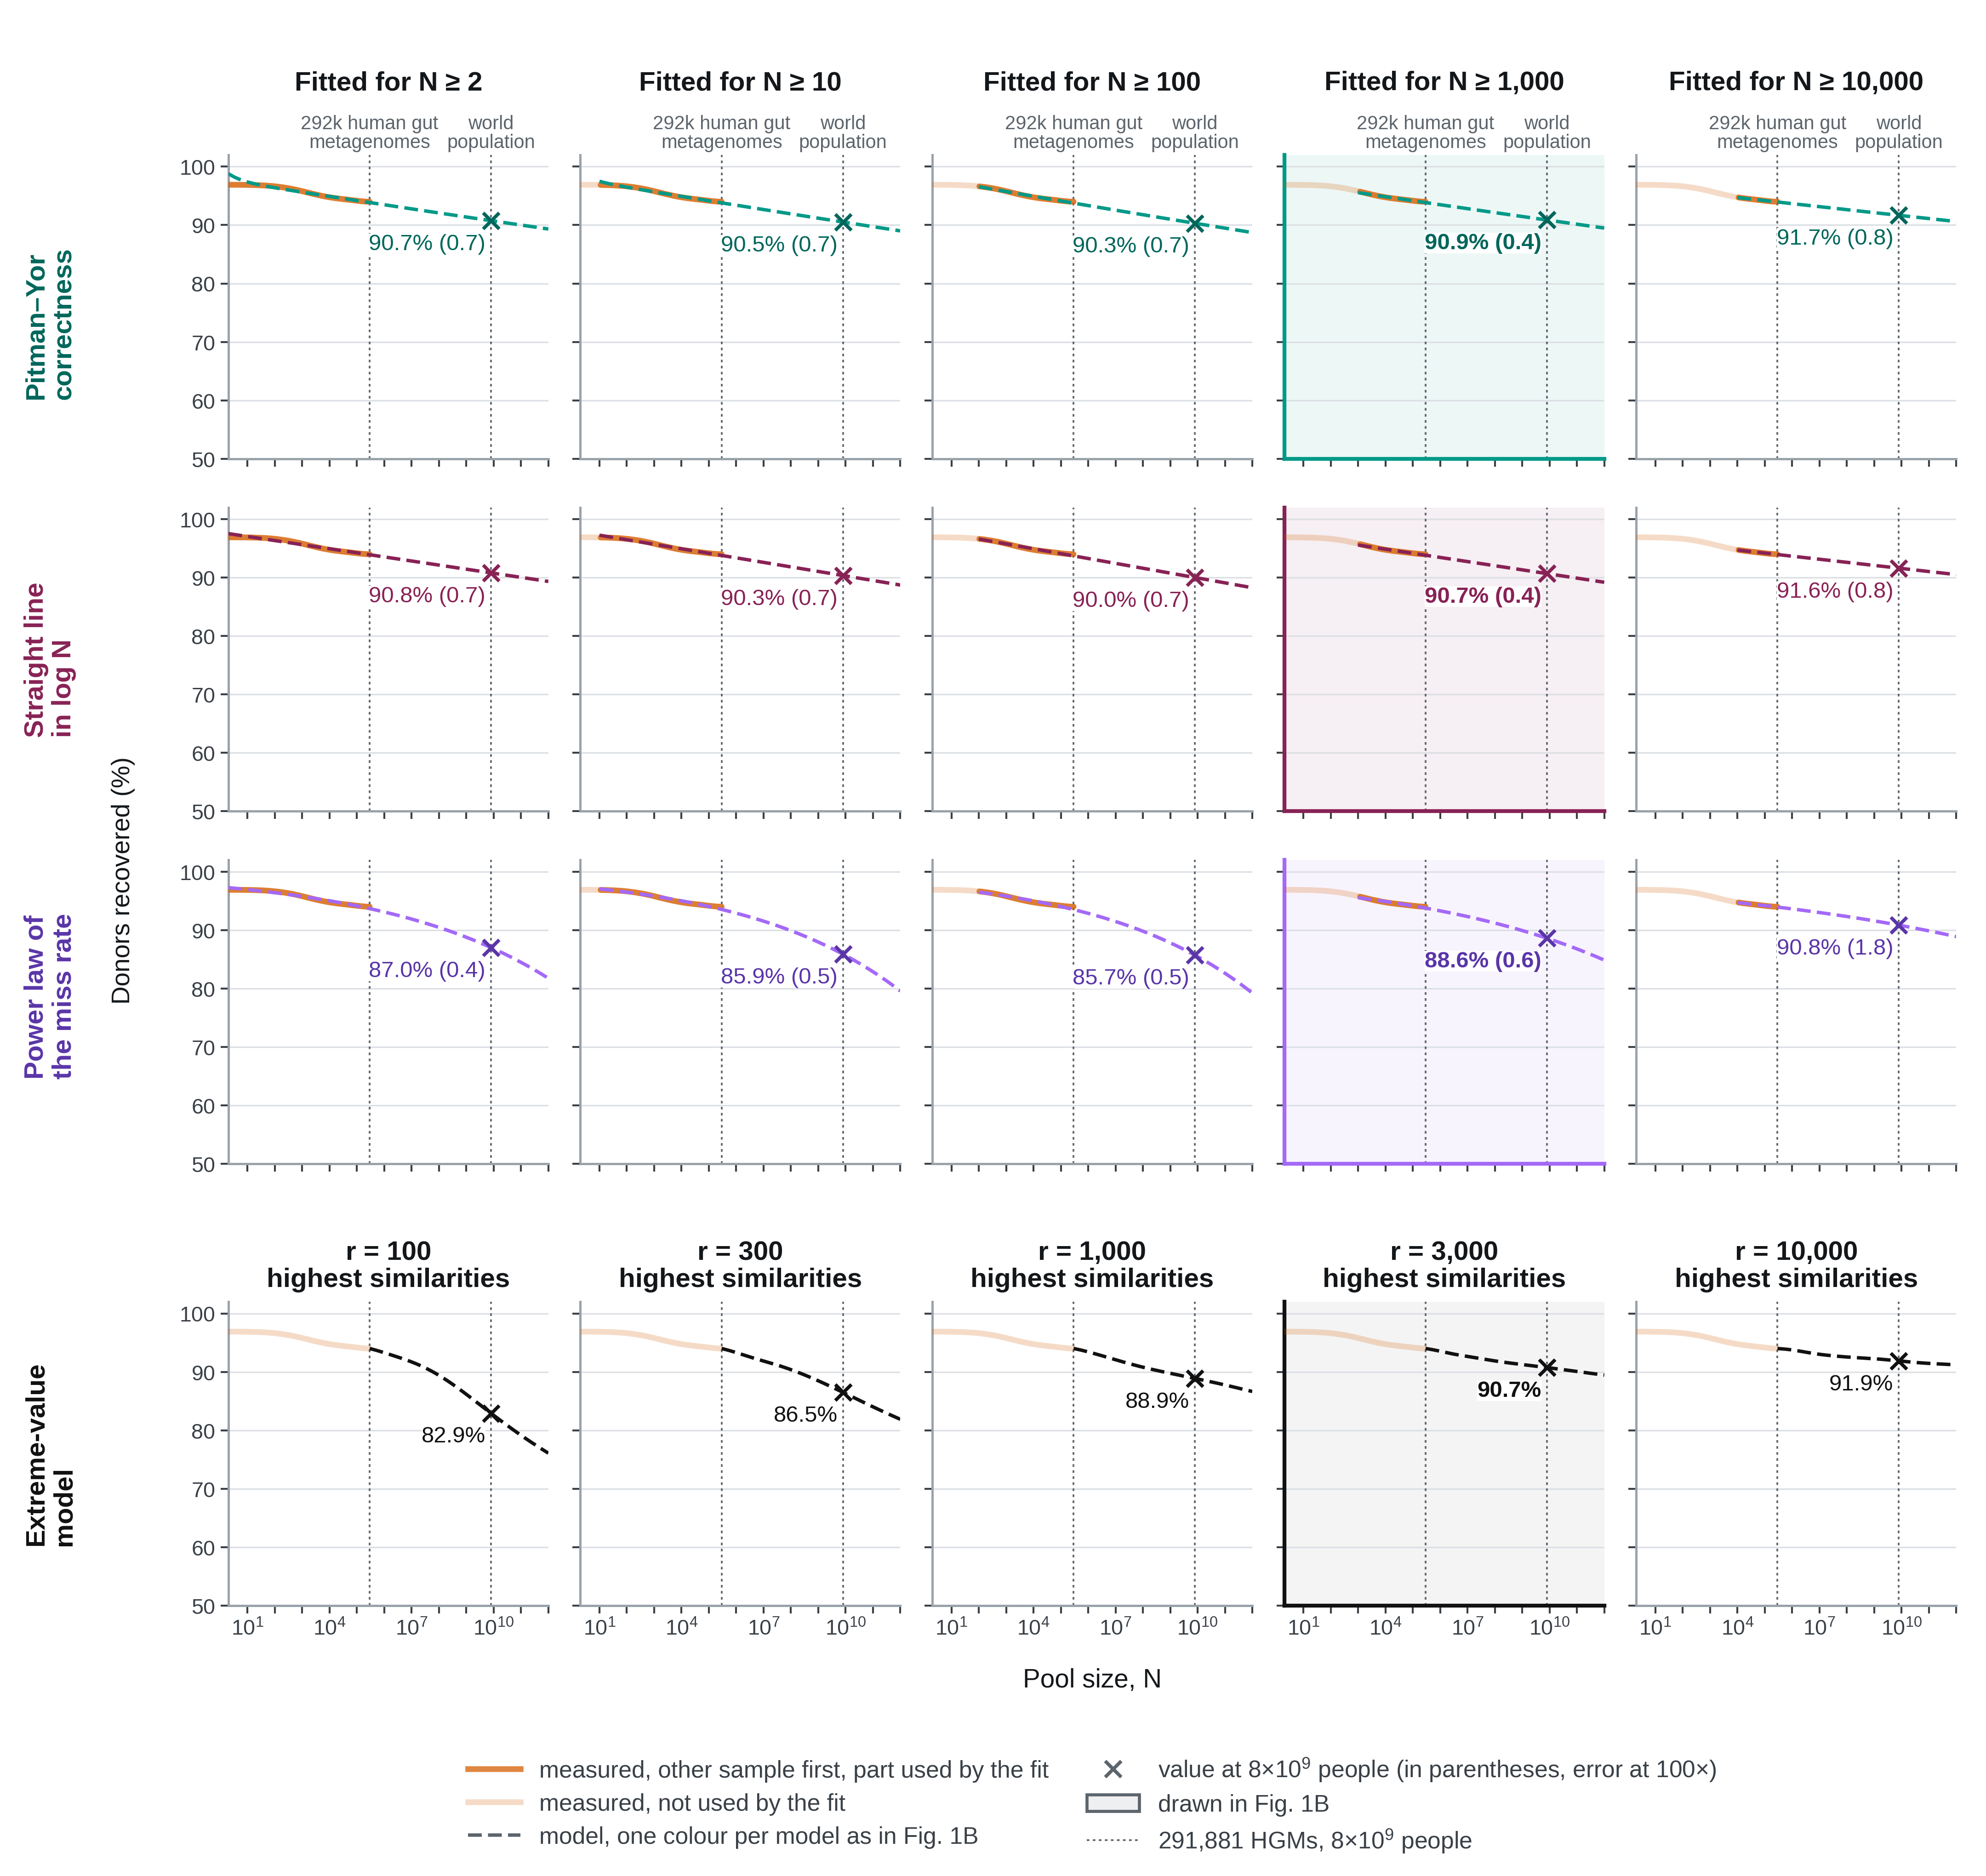
\includegraphics[width=\textwidth,height=0.745\textheight,keepaspectratio]{supplementary_figure5}
\caption[Extrapolations of the recovery curve of Fig. 1B for five fit windows and five tails]{\textbf{Extrapolations of the recovery curve of Fig. 1B for five fit windows and five tails.} Share of the 483 donors whose other sample is first in a pool of $N$ runs, measured in pools drawn from the 291,881 runs of the HGM set (thick line, darker over the pool sizes used by the fit), given by the model up to $10^{12}$ runs (dashed line). First three rows, the three models of Fig. 1B fitted to the measured curve, in the order of its legend; columns, the fit window, from $N$ = 2, 10, 100, 1,000 or 10,000 to 291,881. Last row, the extreme-value model of the similarity tail, which is not fitted to the measured curve and starts from the measured share at 291,881 runs; columns, the tail size $r$, using the 100, 300, 1,000, 3,000 or 10,000 highest similarities of each donor (Supplementary Table 18). Shaded, the fit and the tail drawn in Fig. 1B. Cross and value, the model at the population of the world, $8\times10^9$, with in parentheses, for the first three rows, its root mean square error on thinned HGM sets at 100 times, in percentage points (Supplementary Table 16); at 100 times the windows from 10 and 100 runs give the same thinned fit. Dotted lines, the HGM set and the population of the world.}
\end{figure}

To quantify sampling uncertainty across cohorts and donors, we employ a two-stage cohort-then-donor resampling scheme (Methods), which could also be called a bootstrap method. In each resample, we draw the 7 cohorts with replacement and, for each drawn cohort of size $n_c$, draw $n_c$ donors with replacement from that cohort; we then take the 2.5th and 97.5th percentiles across resamples as the 95\% interval (for the three curve-fitted models we recompute the measured curve and refit each model on every resample, whereas for the extreme-value model we estimate the distribution of tail shapes, $\mathrm{Beta}(a, b)$, again from the donors drawn, each weighted by the number of times it is drawn, which updates the posterior of the shape of every donor, and average the resulting donor probabilities). Resampling cohorts first accounts for between-cohort heterogeneity that an interval treating the 483 donors as independent would ignore. For every model, we select the number of resamples $B$ adaptively by starting at $B = 100$ and doubling $B$ until the Monte Carlo standard error of both interval bounds (estimated from 2,000 draws with replacement among the $B$ resamples) falls below 5\% of the interval width. This 5\% threshold provides a practical compromise: looser stopping rules leave noisy tail quantiles, whereas far tighter rules multiply refitting cost without materially altering the bounds. Supplementary Fig. 6 illustrates both the resulting uncertainty bands (Panels A--C for the curve-fitted models and Panel D for the extreme-value model, showing point extrapolations as dashed lines, 95\% bands as shaded regions and world-population intervals as vertical error bars) and the convergence diagnostics across doubling steps (Panels E--F, showing the relative Monte Carlo standard error falling below the 0.05 threshold and the bounds stabilising). At $8\times10^9$ runs, the resulting 95\% intervals are 81.6--96.6\% for the Pitman--Yor model ($B = 800$), 81.1--97.9\% for the straight line ($B = 800$), 71.1--97.6\% for the power law of the miss rate ($B = 3{,}200$) and 79.5--96.4\% for the extreme-value model ($B = 400$). The power law of the miss rate displays a noticeably wider lower tail and requires a larger $B$ because uncertainty in its log--log slope compounds multiplicatively across 4.4 orders of magnitude, yet even its 95\% lower bound (71.1\%) remains well above the 9--33\% re-identification risk thresholds.

\setcounter{figure}{5}
\begin{figure}[!htbp]\centering
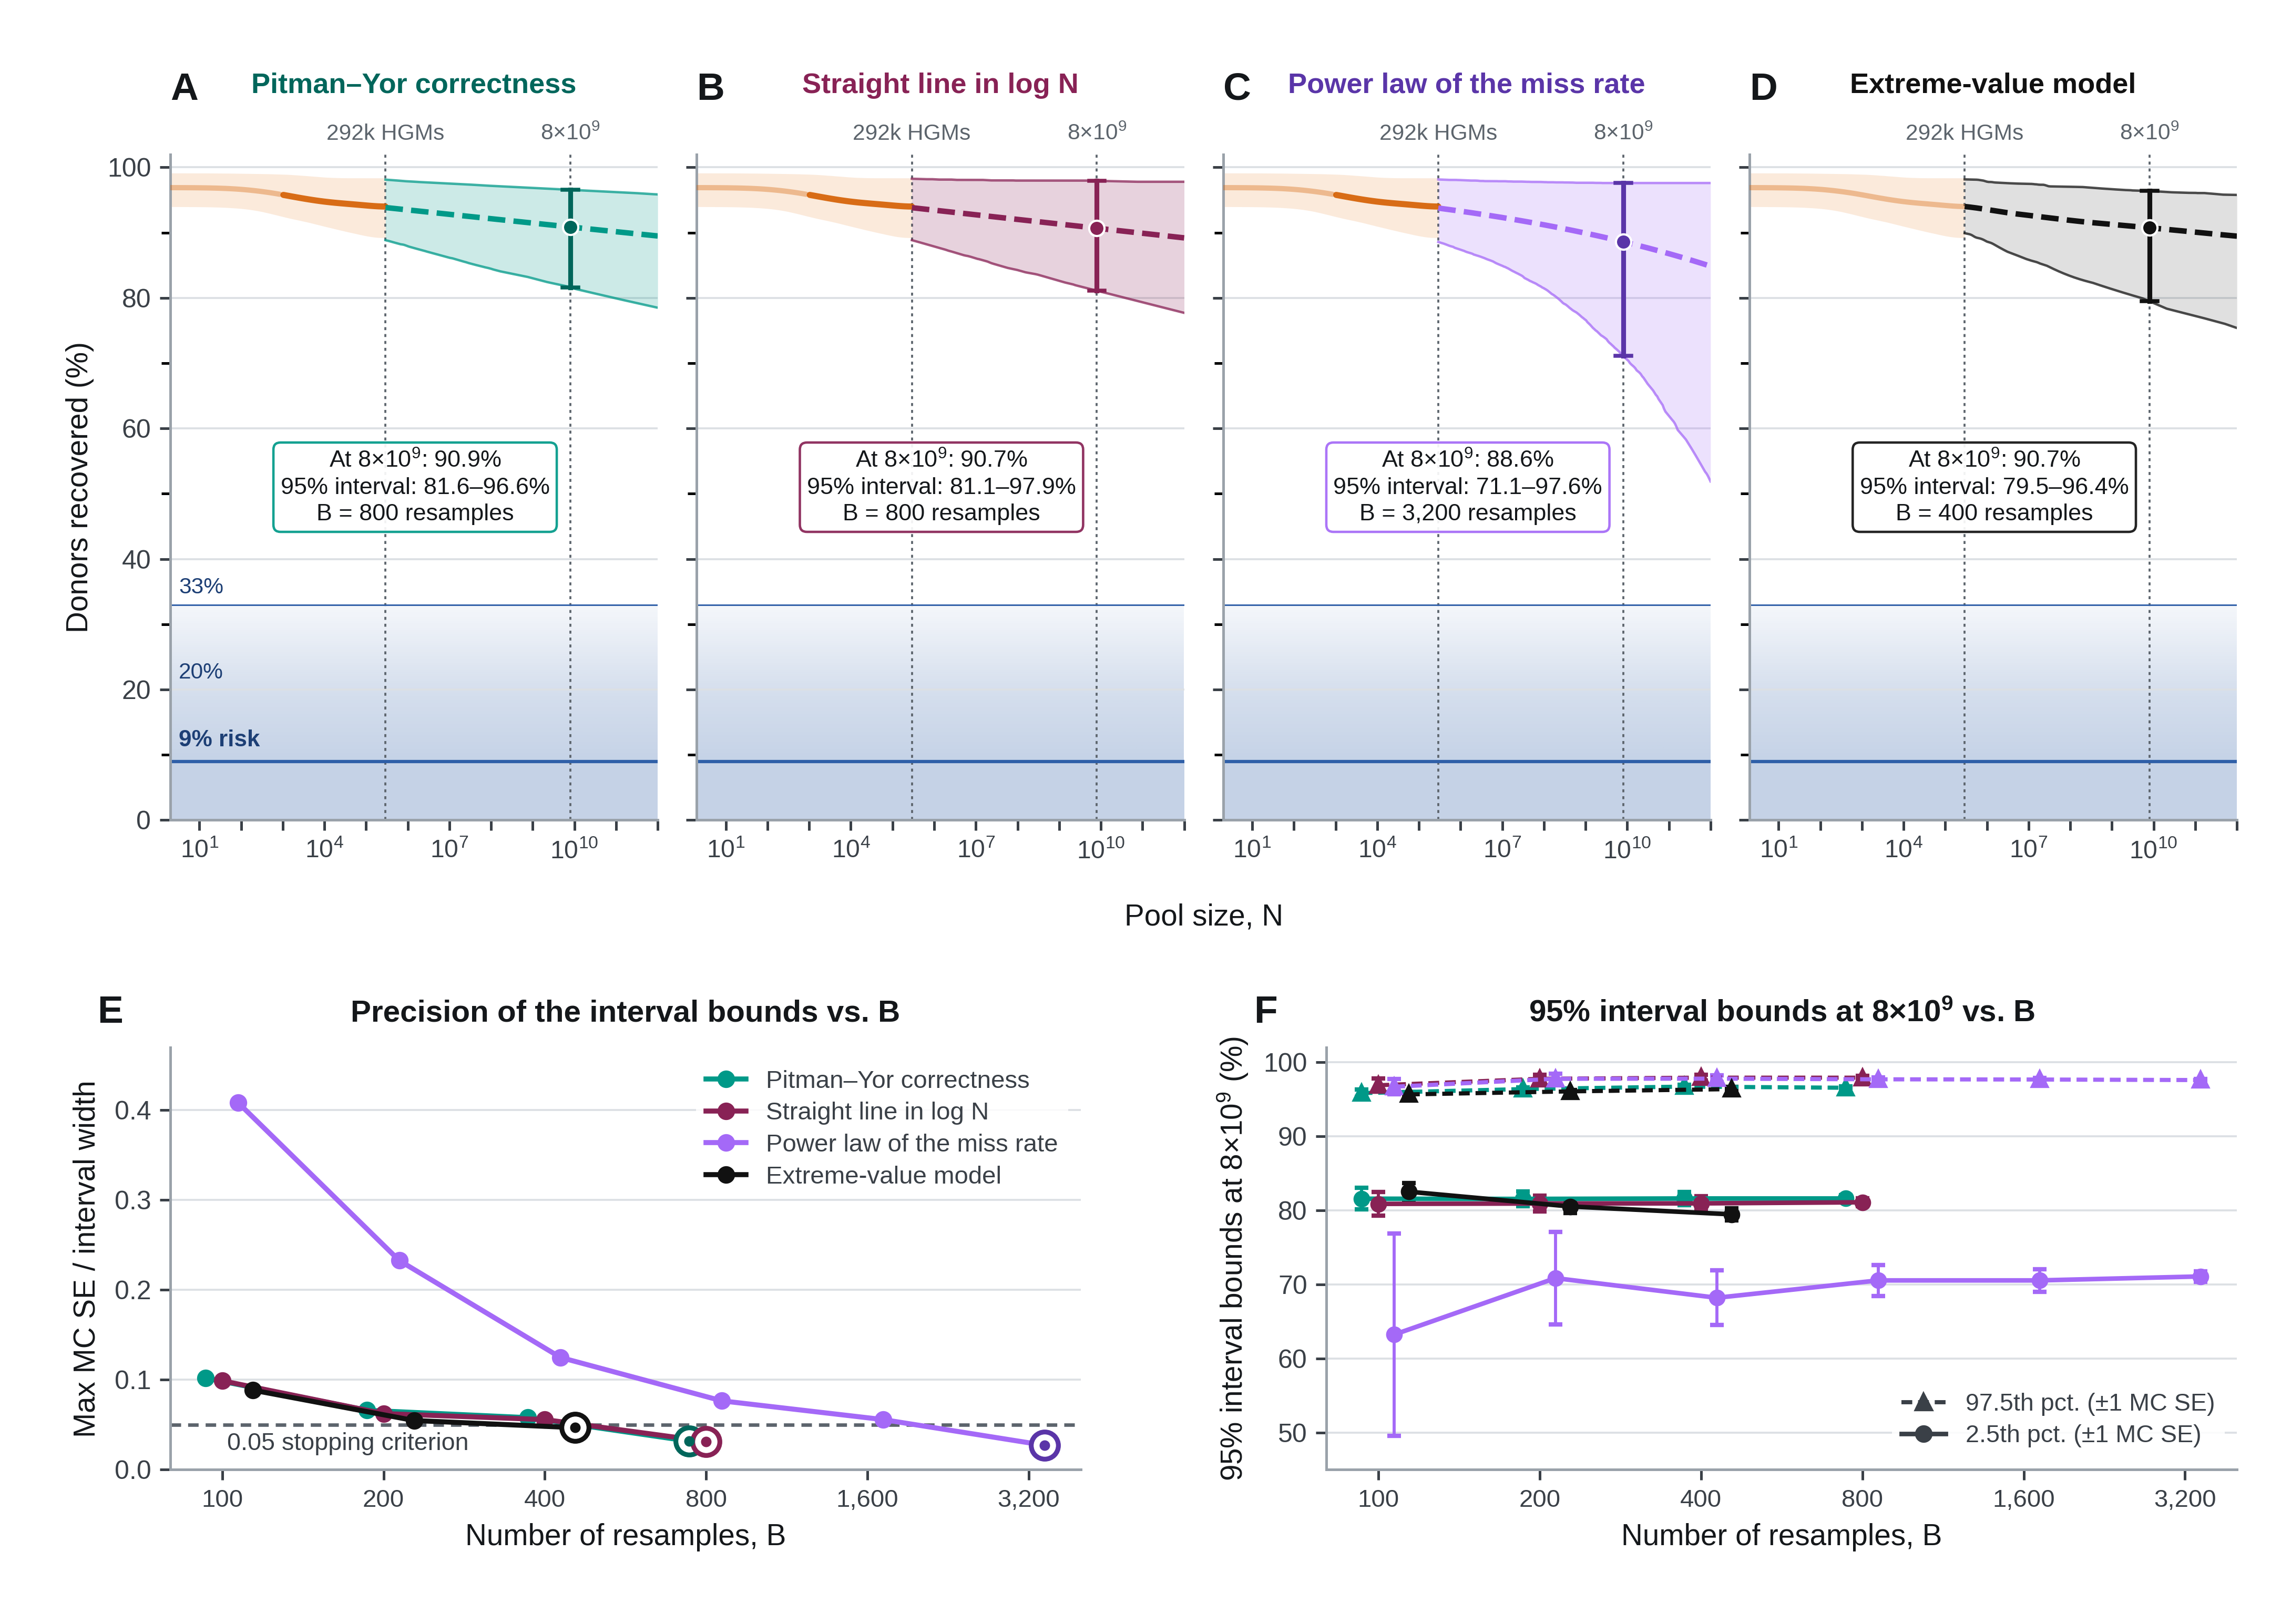
\includegraphics[width=\textwidth,height=0.745\textheight,keepaspectratio]{supplementary_figure6}
\caption[Cohort-then-donor resampling intervals for the four models of Fig. 1B and adaptive selection of $B$]{\textbf{Cohort-then-donor resampling intervals for the four models of Fig. 1B and adaptive selection of $B$.} \textbf{A--D}, Recovery rate against pool size $N$ measured up to 291,881 HGM runs (orange curve and shaded 95\% interval) and extrapolated by the Pitman--Yor correctness model (\textbf{A}), a straight line in $\log N$ (\textbf{B}) and a power law of the miss rate (\textbf{C}), each fitted for $N \ge 1{,}000$, and by the extreme-value model of the similarity tail (\textbf{D}). Dashed lines, point extrapolations; shaded bands, 95\% intervals across $B$ cohort-then-donor resamples; vertical error bars, 95\% intervals at $8\times10^9$ runs. In \textbf{A--C} each model is fitted again on each resample. In \textbf{D} the distribution of tail shapes is estimated again on each resample from the donors drawn, and the resample averages the resulting probabilities of these donors. Blue area and lines, re-identification risk thresholds (9\%, 20\% and 33\%). \textbf{E}, Convergence of the maximum Monte Carlo standard error (from 2,000 draws with replacement among the $B$ resamples) of the 2.5th and 97.5th percentiles at $8\times10^9$ runs relative to interval width as $B$ doubles from 100; ringed points mark the stopping $B$ below the 0.05 threshold. \textbf{F}, Lower (2.5th percentile, solid) and upper (97.5th percentile, dashed) interval bounds at $8\times10^9$ runs with $\pm 1$ Monte Carlo standard error across doubling steps.}
\end{figure}

Beyond thinning accuracy, tuning sensitivity and sampling uncertainty, we verified across all four models that our extrapolations are driven neither by any single cohort nor by the exclusion of the 14 donors removed under the contamination and re-deposit rules, by recomputing the measured rate and the Fig. 1B fits after leaving each cohort out in turn as well as with all 497 donors retained (Supplementary Table 17). Across leave-one-out subsets, the measured recovery rate varies narrowly between 93.4\% and 95.7\%, while world-population extrapolations remain between 86\% and 94\% across the three curve-fitted models and between 87\% and 95\% for the extreme-value model ($r = 3{,}000$); the measured rate is lowest without Mehta, the cohort with the most donors (241 of 483), and highest without Costea, which accounts for 12 of the 29 unrecovered donors. Even when all 497 donors are retained prior to applying the contamination and re-deposit rules, the measured recovery rate stands at 92.0\% and the three curve-fitted extrapolations still range from 74\% to 85\% at $8\times10^9$ runs, while the extreme-value model predicts 88.5\%.

\setcounter{table}{16}
\begin{table}[!htbp]\centering\small\setlength{\tabcolsep}{3.4pt}
\caption[Recovery rate and extrapolations with one cohort left out]{\textbf{Recovery rate and extrapolations with one cohort left out.} Cohorts are named by their curatedMetagenomicData identifiers, in the order of Supplementary Table 11. \textit{Donors}, donors kept. \textit{Recovered}, donors whose other sample is at rank 1 in the HGM set. \textit{At $8\times10^9$}, the three fits drawn in Fig. 1B (bold in Supplementary Table 16), namely the Pitman--Yor correctness model, the straight line in $\log N$ and the power law of the miss rate, made again on the measured curve of the donors kept, and the extreme-value model of the similarity tail (bold in Supplementary Table 18), made again on the donors kept, as shares in \%. \textit{None}, all the 483 donors. Last row, all the 497 donors of the cohorts kept, with the 14 that the rules of contamination and re-deposit remove (Supplementary Note 1).}
\begin{tabular}{lrrrrrr}
\toprule
 & & & \multicolumn{4}{c}{At $8\times10^9$ (\%)} \\
\cmidrule(lr){4-7}
Cohort left out & Donors & Recovered (\%) & Pitman--Yor & Straight line & Power law & Extreme value \\
\midrule
None & 483 & 454 (94.0) & 90.9 & 90.7 & 88.6 & 90.7 \\
CosteaPI\_2017 & 399 & 382 (95.7) & 93.9 & 93.7 & 92.7 & 94.5 \\
MehtaRS\_2018 & 242 & 226 (93.4) & 89.5 & 89.3 & 86.3 & 87.0 \\
HansenLBS\_2018 & 439 & 412 (93.8) & 90.4 & 90.2 & 87.7 & 90.3 \\
RaymondF\_2016 & 459 & 431 (93.9) & 91.0 & 90.8 & 89.1 & 91.1 \\
HMP\_2019\_ibdmdb & 435 & 407 (93.6) & 90.1 & 89.9 & 87.5 & 90.2 \\
Heitz-BuschartA\_2016 & 470 & 441 (93.8) & 90.6 & 90.4 & 88.3 & 90.5 \\
Bengtsson-PalmeJ\_2015 & 454 & 425 (93.6) & 90.3 & 90.1 & 87.9 & 90.2 \\
\midrule
None, with the donors & 497 & 457 (92.0) & 85.3 & 85.0 & 74.1 & 88.5 \\
removed by the two rules & & & & & & \\
\bottomrule
\end{tabular}
\end{table}

Full numerical diagnostics across all five tails of the extreme-value model appear in Supplementary Table 18. Taken together, these validation, sensitivity, resampling and cohort-removal checks confirm that the high extrapolated recovery rates are consistent across model families and robust to sampling variation and data selection, remaining well above the 9--33\% re-identification risk thresholds in every scenario tested.

\setcounter{table}{17}
\begin{table}[!htbp]\centering\small\setlength{\tabcolsep}{3.5pt}
\caption[Extreme-value model of the similarity tail for five tails and test on thinned HGM sets]{\textbf{Extreme-value model of the similarity tail for five tails and test on thinned HGM sets.} Generalised Pareto shape $\xi_i \in [-0.5, 0.5]$. \textit{Tail}, the number of highest similarities of the runs of other people used for each donor, and their share of these runs; bold, the tail drawn in Fig. 1B. \textit{Mean shape}, the mean of the distribution of shapes. \textit{Recovered}, share of the 483 donors whose other sample is first according to the model in a pool of $10^7$ runs and of $8\times10^9$ runs, the size of the population of the world, with its 95\% interval on 400 resamples of cohorts, then donors. Test, each run of other people is kept with probability $f$ (0.1, 0.03, 0.01) and the model is fitted on the thinned data alone with the same share of the runs of other people in the tail. \textit{Mean error} and \textit{RMSE}, mean and root mean square, over 400 thinnings, of the recovery rate that the model predicts at 291,881 runs minus the measured share (94.0\%), in percentage points, at 10, 33 and 100 times the thinned HGM set. --, a tail of fewer than ten similarities in the thinned HGM set, which is not fitted. Last row, constant-rate baseline, the share measured in the thinned HGM set itself taken as the prediction.}
\begin{tabular}{rrrrrcrrrrrr}
\toprule
\multicolumn{2}{c}{Tail} & & \multicolumn{3}{c}{Recovered (\%)} & \multicolumn{3}{c}{\makecell[cb]{Mean error\\(percentage points)}} & \multicolumn{3}{c}{\makecell[cb]{RMSE\\(percentage points)}} \\
\cmidrule(lr){1-2}\cmidrule(lr){4-6}\cmidrule(lr){7-9}\cmidrule(lr){10-12}
Runs & \% & \makecell[cb]{Mean\\shape} & At $10^7$ & At $8\times10^9$ & Interval & $\times$10 & $\times$33 & $\times$100 & $\times$10 & $\times$33 & $\times$100 \\
\midrule
100 & 0.034 & $-$0.06 & 91.7 & 82.9 & 67--92 & $-$0.86 & -- & -- & 0.90 & -- & -- \\
300 & 0.10 & $-$0.07 & 91.9 & 86.5 & 69--94 & $-$0.38 & -- & -- & 0.41 & -- & -- \\
1,000 & 0.34 & $-$0.09 & 92.1 & 88.9 & 73--95 & $-$0.14 & $-$0.28 & $-$0.91 & 0.18 & 0.34 & 1.07 \\
\textbf{3,000} & \textbf{1.0} & \textbf{$-$0.11} & \textbf{92.6} & \textbf{90.7} & \textbf{79--96} & \textbf{+0.02} & \textbf{+0.04} & \textbf{$-$0.07} & \textbf{0.12} & \textbf{0.14} & \textbf{0.23} \\
10,000 & 3.4 & $-$0.14 & 93.0 & 91.9 & 84--97 & +0.16 & +0.24 & +0.31 & 0.20 & 0.28 & 0.35 \\
\midrule
\multicolumn{3}{l}{Constant-rate baseline} & -- & -- & -- & +0.45 & +0.80 & +1.34 & 0.48 & 0.83 & 1.36 \\
\bottomrule
\end{tabular}
\end{table}

\subsection*{Scope and limitations of the extrapolations}\addcontentsline{toc}{subsection}{Scope and limitations of the extrapolations}

Four methodological limitations apply across these extrapolations and warrant caution when interpreting predictions at population scale. First, every model assumes that newly added runs drawn into larger pools follow the same similarity distribution as the HGM set; outliers far above the empirical distribution, such as close relatives or untracked re-deposits of the donor, are not represented. Second, extrapolating to the world population spans roughly 27,000 times the HGM set, whereas thinned-pool validation covers at most 100-fold growth (a regime in which the smallest tails of the extreme-value model retain too few excesses to be fitted). Third, behaviour far beyond $8\times10^9$ runs remains sensitive to parametric tail assumptions (including, for the extreme-value model, the tendency of negative GPD shape parameters to induce finite upper endpoints that can arise from finite-threshold samples of unbounded distributions such as Gaussian tails), so these curves should not be extrapolated arbitrarily beyond human population scale. Fourth, the reported 95\% intervals capture cohort and donor sampling uncertainty only; for the extreme-value model they include the re-estimation of the distribution of tail shapes on every resample, but not any dependence among the non-match similarities to a given query, which its likelihood treats as conditionally independent.


\FloatBarrier
\section*{Supplementary Note 4. Thresholds of re-identification risk}\addcontentsline{toc}{section}{Supplementary Note 4. Thresholds of re-identification risk}

The main text compares the recovery rate with the thresholds of re-identification risk advised for the release of clinical data. This Note explains how this risk is measured, how our recovery rate relates to this measure, and where the values of the thresholds come from.

The thresholds come from the methods used to anonymise clinical data before their release, in the Institute of Medicine report\cite{iom2015} (appendix B by El Emam and Malin) and the guidance of the European Medicines Agency\cite{ema}. These methods give each record of a data set a probability of being re-identified. Records that share the same values of the indirectly identifying variables cannot be told apart and form a group. The re-identification probability of a record is 1 divided by the number of individuals in its group. For example, a record in a group of 11 has a probability of 1 in 11, or approximately 0.09, while a record alone in its group has a probability of 1. For the whole data set, the maximum risk is generally the highest probability among its records but the average of these probabilities (the average risk) is also considered. Both texts mentioned above retain the maximum risk for a public release. According to the report of the Institute of Medicine, the reason is that no contract binds the recipient of public data and that an adversary can target the record that is easiest to re-identify.

In our analysis the microbiome plays the role of the indirectly identifying variables. A recovered donor is analogous to a record alone in its group, since no record from another individual in the set is more similar to the query than the donor's other sample. This sample can thus be unambiguously singled out. The recovery links the two samples of this donor with a probability of 1, and a donor that is not recovered counts for 0. The recovery rate is the mean of these values over the donors and is therefore an average risk. This holds for the rate measured with the full HGM set, 454 of 483 donors or 94.0\%, and for the rates extrapolated to the world population (Supplementary Note 3). As mentioned, the maximum re-identification risk is the highest individual probability of re-identification, so recovering even a single donor is theoretically sufficient to bring it to 1. Our analysis using the full HGM set yields a maximum risk of 1 and an average risk of 0.94, both exceeding the 0.09 threshold (see below). Although thresholds for public data release are generally based on maximum risk, in this article, we report the average across donors because a maximum risk of 1 could arise from a single donor, whereas the average demonstrates that this risk is a widespread property of adult gut microbiomes.

A threshold on the maximum risk is the inverse of the smallest group that a data custodian accepts, called the minimum cell size. Data custodians, in particular the government agencies that report statistics, have long applied such minimum sizes to what they release, and the appendix of the report of the Institute of Medicine reviews them. The most common minimum is 5, a probability of 1 in 5 or 0.2, but it was not recommended. Some public health offices use 3 (0.33). Larger minima are in use, such as 11 in the United States (0.09) and 20 in Canada (0.05), and the largest that this review found is 25 (0.04). The review states that no threshold is agreed upon, that the lowest probabilities are used for public releases, and that a minimum of 20 is appropriate for them.

The minimum of 11 is the rule of the Centers for Medicare \& Medicaid Services, which allow no cell smaller than 11 to be displayed from their data\cite{cms2020}. The European Medicines Agency advises a threshold of 0.09 on the maximum risk for the clinical reports that it publishes. It bases this value on the recommendations made in the report of the Institute of Medicine and on the precedents for the public release of health data, and an applicant may justify another value. Health Canada encourages the same threshold, which it equates to a smallest group of 11 patients who share the same indirectly identifying values\cite{healthcanada2019}.

Thresholds used in practice range from 33\% to 4\%, and the traditional 20\% is used more often for trusted recipients than for public release\cite{iom2015,elemam2011b,elemam2013}. The fading area of Fig. 1B spans 33\% to 9\%.

One of the main principles of many privacy laws is that identification does not have to be proved and that it is anonymisation that has to be proved (principle of privacy by default, recognised in various data protection frameworks, including those of the European Union, the United Kingdom, Switzerland and Kenya). Recovering a donor establishes a link between two metagenomic samples from the same individual, even when they are deposited under different identifiers. This ability, known as \textit{linkability}, is one of the three risks that anonymisation must address\cite{wp29} to consider data as anonymous. The European Data Protection Board is working on an updated version of the criteria. These new guidelines\cite{edpb2026} also rule the absence of linkage between records as a criterion for assessing anonymity. This criterion is particularly important for publicly released data, which can be linked by anyone with the necessary means (in our case effortlessly thanks to the Faure \textit{et al.} web service). Our results demonstrate that such linkage is already achievable using publicly accessible tools, directly challenging the assumption that publicly released gut metagenomic sequences can be considered anonymous in the European Union and in countries sharing the same kind of rule.

\clearpage

















\FloatBarrier
\bibliographystyle{sn-nature}
\bibliography{references}
\end{document}
